% !TeX root=../../../main.tex

\chapter{نتایج تجربی}

تا به اینجا مسئله پیش رو و ابعاد پیچیدگی آن مشخص شده است. همچنین حوزه‌های درگیر و مفاهیم مرتبط را نیز بازگو شده است و پس از آن مفروضات و روش‌های مختلف مرتبط برای حل مسئله بررسی شد. 
در نهایت در فصل گذشته نیز رویکرد پیشنهادی در این پایان‌نامه برای پاسخ به این مسئله ارائه گشت. حال در این فصل قصد داریم تا در عمل روش پیشنهادی خود را بسنجیم و نتایج حاصل از آن را مشاهده نماییم.
\\
به همین منظور در این فصل ابتدا پایگاه داده‌ای مجازی تهیه می‌کنیم و در ادامه نحوه استفاده از روش پیشنهادی و آموزش و استفاده از شبکه طراحی شده را خواهیم گفت. پس از آن به نتایج بدست آمده بر روی پایگاه داده مصنوعی می‌پردازیم و حالات مختلف آن را مورد ارزیابی قرار می‌دهیم و در نهایت نتیجه اجرای روش پیشنهادی خود را بر روی یک داده حقیقی مشاهده خواهیم نمود.

\section{پایگاه داده‌های ورودی}
قبل از اینکه وارد روش پیشنهادی شویم به تشریح وردی‌های مسئله و داده‌هایی که مورد استفاده قرار خواهیم داد می‌پردازیم.
داده‌های ورودی برابر ماتریس $D_{m\times n}$ می‌باشد که بعد اول $M$ برابر با ژن‌ها و بعد دوم $N$ برابر سلول‌های نمونه‌برداری شده می‌باشد. در هر خانه $d_{i,j}$ یک بردار داده قرار دارد که حاوی اطلاعات ژن $j$ در سلول $i$ می‌باشد.

\subsection[پایگاه داده مصنوعی]
{پایگاه داده مصنوعی
	\LTRfootnote{Synthetic Dataset}
}

با توجه به این نکته که از درخت فیلوژنی حقیقی\LTRfootnote{Ground-truth Phylogeny Tree} داده‌های حقیقی موجود اطلاعی نداریم، به سراغ ساخت پایگاه‌ داده مصنوعی می‌رویم. با استفاده از این پایگاه داده مصنوعی می‌توانیم در مورد روش‌هایی که در ادامه بیان خواهیم کرد یک معیار ارزیابی نسبتا مناسبی داشته باشیم و تا حدودی از مشکلات روش‌های پیشنهادی آکاه شویم و به تصحیح آن بپردازیم. برای ساخت پایگاه داده مصنوعی که همان ماتریس ورودی $D_{m\times n}$ می‌باشد، از دو روش مختلف با دو فرض مختلف استفاده خواهیم کرد که در ادامه به تشریح هر کدام خواهیم پرداخت.


در ادامه جدول
\ref{tab:ch_er:datasetIndices}
را برای معرفی اندیس‌های بکار گرفته شده در روابط مربوط به تولید پایگاه‌داده مجازی بیان می‌نماییم.
\begin{table}[ht]
	\caption{اندیس‌های به کار رفته در تولید پایگاه داده مجازی}
	\label{tab:ch_er:datasetIndices}
	\centering
	\onehalfspacing
	\begin{tabularx}{0.9\textwidth}{|r|X|}
		\hline
		$D$	& ماتریس داده نویزی در دسترس که مقادیر $0$، $1$ و $3$ (به عنوان داده از رفته) در آن قرار دارد \\
		\hline
		$E$	& ماتریس داده حقیقی بدون نویز که به دنبال آن هستیم \\
		\hline
		$T$	& درخت فیلوژنی جهش‌ها \\
		\hline
		$C$ & پروفایل تعداد کپی نمونه‌ها \\
		\hline
		$N$	& تعداد سلول‌های نمونه \\
		\hline
		$M$	& تعداد جهش‌ها \\
		\hline
		$\alpha$ & نرخ خطای \gls{falsepositive} \\
		\hline
		$\beta$	& نرخ خطای \gls{falsenegative} \\
		\hline
		$\zeta$ & پارامتر تعیین‌کننده میزان چاقی و لاغری درخت‌ \\
		\hline
		$\gamma$ & پارامتر تعیین‌کننده میزان ادغام جهش‌ها در یک گره (عدم مشاهده نمونه بینشان) \\
		\hline
		$\psi$ & تعیین‌کننده احتمال فقدان یک جهش \\
		\hline
		$\vartheta$ & تعیین‌کننده میزان تاثیر در وقوع فقدان متناسب با فاصله از وقوع جهش \\
		\hline
		$\varrho$	& احتمال کاهش تعداد کپی بدون از دست رفتن جهش \\
		\hline
	\end{tabularx}
\end{table}
\\
برای ایجاد پایگاه داده در این حالت ابتدا درختی تصادفی با پارامترهای $\zeta, n$ ایجاد می‌کنیم که $n$ تعداد ژن‌ها (جهش‌ها) بوده و $\zeta$ عددی در بازه $(0, \infty)$ است که یک پارامتر کنترلی است که وظیفه‌اش کنترل کلی تعداد نسل‌های مختلف را از یک جمعیت در درخت فیلوژنی می‌باشد.
حال برای تولید پایگاه داده مصنوعی به ترتیب چهار گام زیر باید انجام شود.
\begin{itemize}
	\item ایجاد یک درخت فیلوژنی تصادفی
	\item مشخص کردن برخی ژن‌ها برای حذف در ادامه و تولید پروفایل تعداد کپی
	\item تبدیل درخت فیلوژنی حاصل به ماتریس اطلاعات سلول-ژن ($E$)
	\item اضافه کردن نویز به ماتریس $E$ و تبدیل آن به ماتریس نویزی $D$
\end{itemize}
در ادامه هر بخش به صورت جداگانه به تفضیل شرح داده خواهد شد.

\subsubsection{ساخت درخت تصادفی}
برای ساخت درخت تصادفی از دو روش مختلف استفاده شده است که هرکدام جداگانه توضیح داده شده است.
\vspace{20pt}
\\
\textbf{روش اول: با استفاده از\gls{randombinarygenealogicaltree}}
\\
در این روش همان‌گونه که از نام آن مشخص است با استفاده از درخت تصادفی دودویی ژنولوژی به ساخت ماتریس داده ورودی مسله می‌پردازیم که برای ساخت این دادگان از فرض‌های که در ادامه آمده است استفاده خواهیم کرد. 

در مرحله اول که ساخت درخت است به این صورت عمل میکنیم که به تعداد $n$ گونه (سلول) در نظر می‌گیریم. سپس به ترتیب مراحل زیر را انجام می‌دهیم تا به درخت تصادفی مورد نظر برسیم.
\begin{itemize}
	\item به هر کدام از $n$ گونه متمایز در ابتدا وزن $w_i=1$ را اختصاص می‌دهیم که متناسب با احتمال انتخاب هر گونه در مراحل بعدی خواهد بود.
	\item برای هر گونه ‌$i$ تابع جرم احتمال را در ادامه به صورت $F_i=\frac{w_i}{\sum_{i=1}^{n}w_i}$ در نظر میگیریم
	\item با استفاده از $F$ دو گونه متمایز $u, v$ را انتخاب می‌کنیم و به هم متصل می‌کنیم
	\item به جای دو گونه $u, v$ یک گونه جدید $uv$ با وزن $w_{uv}=\frac{w_u+w_v}{\sqrt[4]{\zeta}}$ را قرار می‌دهیم.
	\item تعداد گونه‌ها یک واحد کم شده است. بررسی می‌کنیم اگر تعداد گونه‌های باقی‌مانده از $2$ کمتر باشد درخت تصادفی ساخته شده است و پایان کار است. در غیر این صورت به مرحله اول بازمی‌گردیم.
\end{itemize}
پارامتر $\zeta$ به گونه‌ای کنترل‌کننده میزان ناپایداری در طی نسل‌ها می‌باشد. بطوریکه نمونه‌ای از نتایج مقادیر مختلف آن برای $n=20$ در شکل \ref{fig:dsismn20} آورده شده است. پس از ساخت درخت تصادفی به سراغ مرحله بعد یعنی تبدیل درخت به ماتریس ژن-سلول $E$ می‌رویم.
\begin{figure}[!ht]
	\centering
	\subfloat[$\zeta=0.2$]{
			\centering
			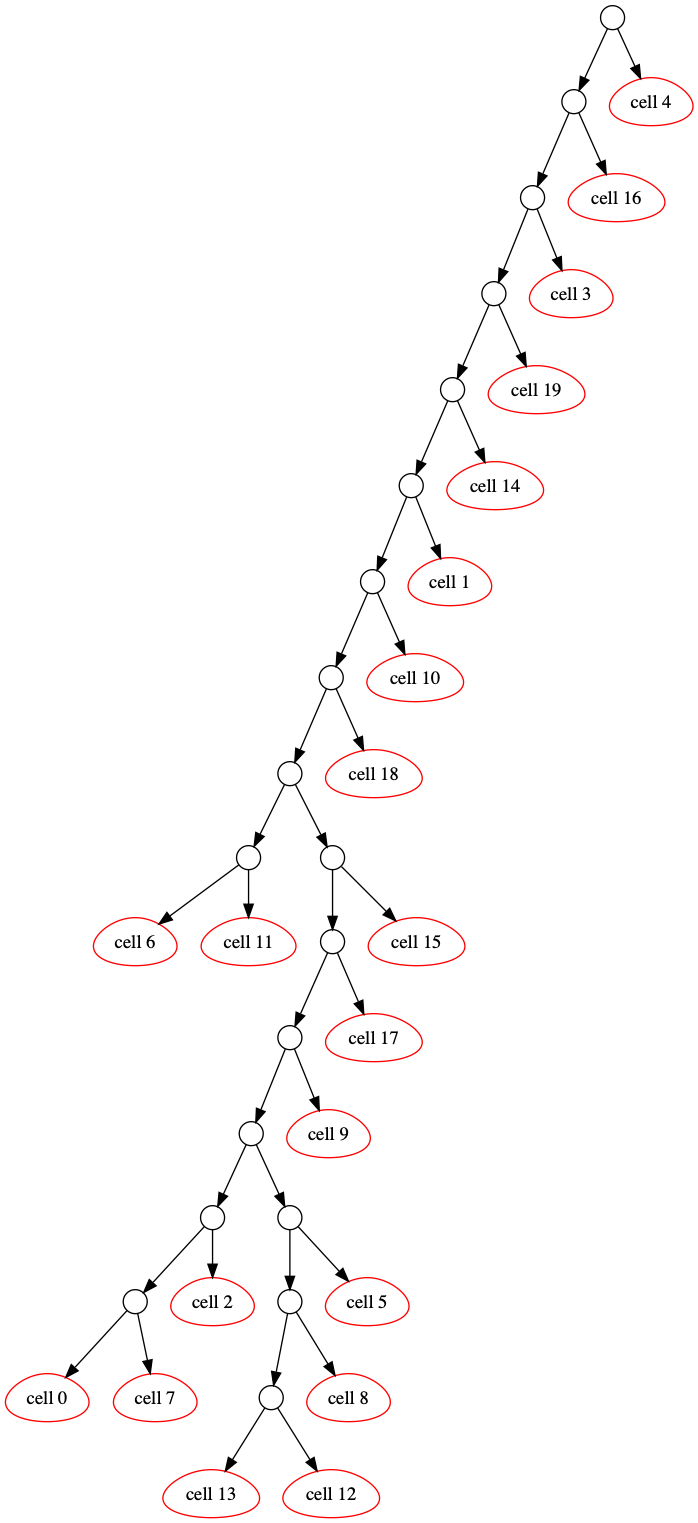
\includegraphics[width=0.48\textwidth, height=0.42\textheight]{img/dataset/s/n20_zeta02}
			\label{fig:dstn20zeta0.2}
	}
	\hfill
	\subfloat[$\zeta=1.0$]{
			\centering
			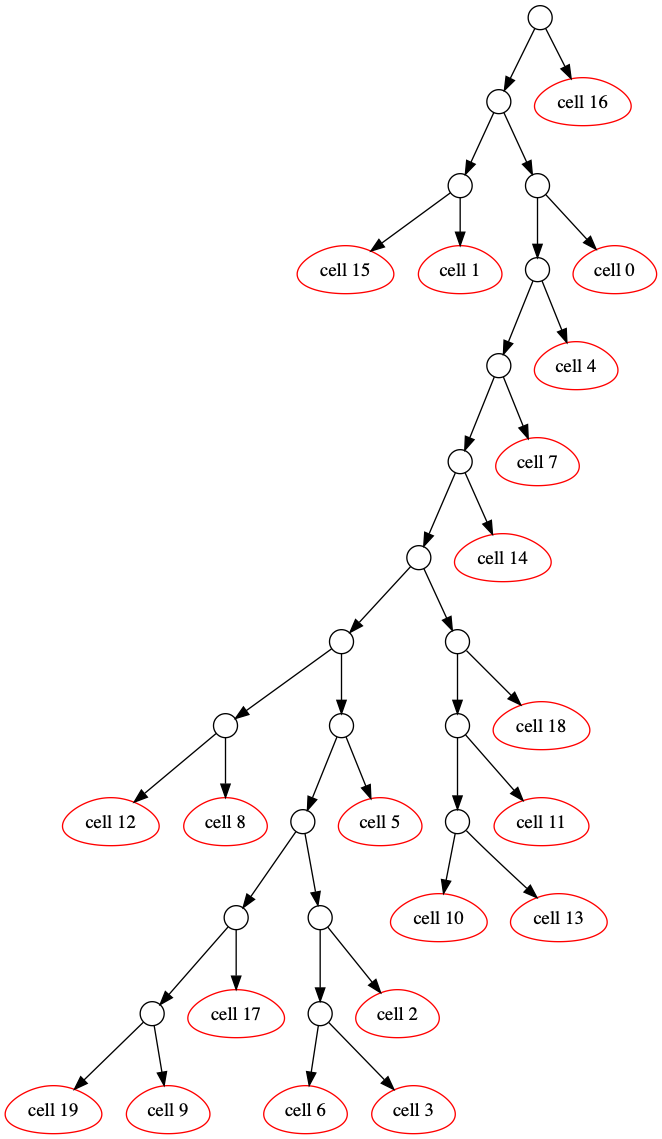
\includegraphics[width=0.48\textwidth, height=0.42\textheight]{img/dataset/s/n20_zeta1}
			\label{fig:dstn20zeta1}
	}
	\hfill
	\vskip\baselineskip
    \subfloat[$\zeta=8$]{
    	\centering
    	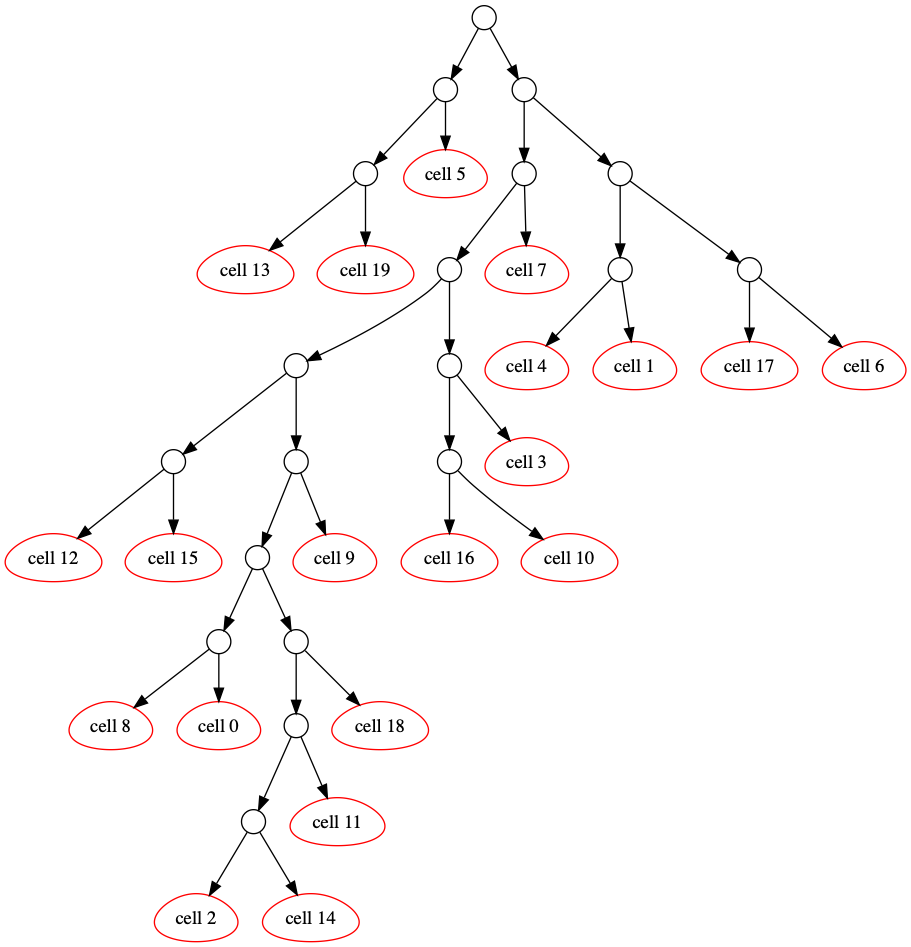
\includegraphics[width=0.38\textwidth, height=0.27\textheight]{img/dataset/s/n20_zeta8}
    	\label{fig:dstn20zeta8}
    }
	\hfill
	\subfloat[$\zeta=100$]{
		\centering
		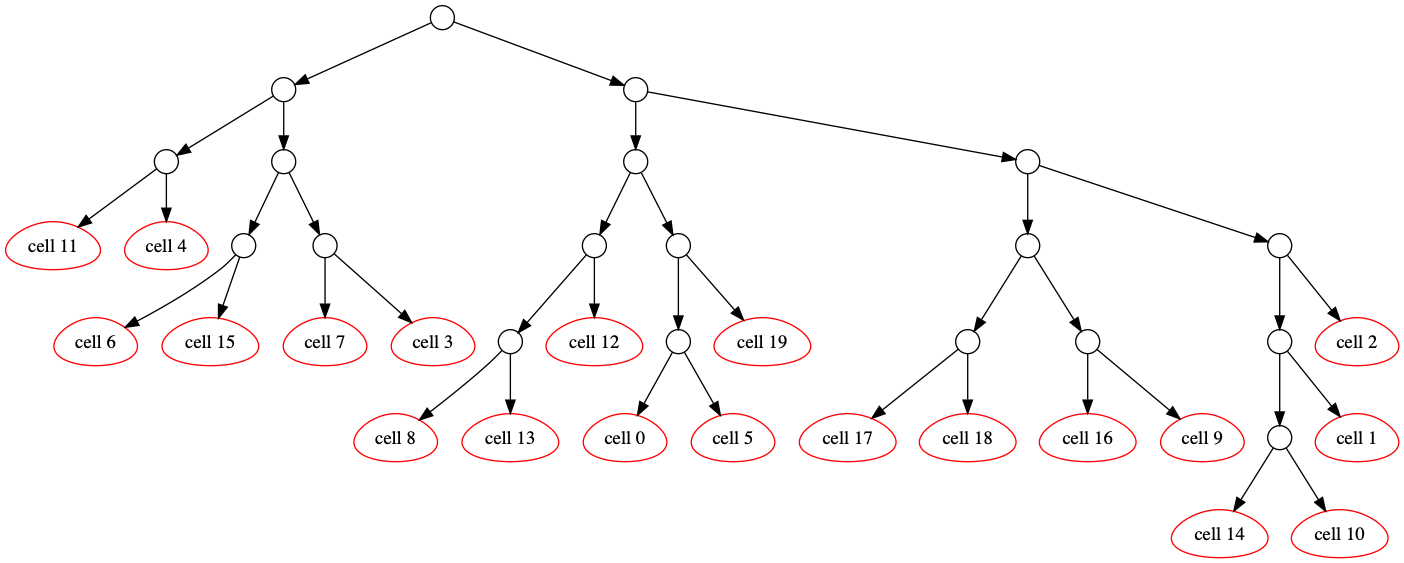
\includegraphics[width=0.58\textwidth, height=0.22\textheight]{img/dataset/s/n20_zeta100}
		\label{fig:dstn20zeta100}
	}
	\caption{درخت فیلوژنی تصادفی تولید شده برای $n=20$ و $\zeta$های مختلف}
	\label{fig:dsismn20}
\end{figure}
\\
در ادامه با توجه به اینکه تعداد دلخواه جهش‌ها چه عددی بوده است یکی از گام‌های زیر را برمی‌داریم.

\begin{itemize}
	\item اگر تعداد جهش‌ها $M>N$ بوده باشد در آن صورت به صورت تصادفی به تعداد دفعات اختلاف یکی از انشعاب‌ها در درخت را به صورت تصادفی انتخاب کرده و آن جهش اضافه شده را تا تمامی نوادگان پیش خواهیم برد.
	\item اگر تعداد جهش‌ها $M<N$ بوده باشد آنگاه مجددا به اندازه تعداد اختلاف انشعاب‌هایی را انتخاب کرده و این بار جهش در آن انشعاب را تا تمامی نوادگان حذف می‌کنیم.  
\end{itemize}
به این ترتیب تمامی سلول‌ها را با تعداد جهش‌های انتخابی خواهیم داشت. در نهایت برای اخرین تغییر در جهش‌ها می‌توان یک گام دیگر برداشت که آن تولید یه عدد تصادفی کوچکتر از $\frac{M}{2}$ است که به آن تعداد می‌توان جهش‌های موجود را از انشعابی برداشت و بر روی انشعابی دیگر قرار داد. با این کار ممکن است تعداد جهش‌ها در انشعاب‌های مختلف تغییر کند و چه بسا به مدل‌های واقعی نزدیکتر شود که البته در این پایان‌نامه از گام آخر صرف‌نظر کرده‌ایم.
\\
حال کار ما با پخش تصادفی جهش‌ها در پایگاه‌داده مجازی پایان یافته است. تا به اینجا ما در فرض خود از هر نمونه جمعیت مختلف یک سلول داشته‌ایم. اما  در بعضی مواقع در پایگاه داده‌های واقعی ممکن است از یک جمعیت بیش از یک نمونه وجود داشته باشد که البته این امر لزوما درست نیست به این دلیل که بعد از افزوده شدن نویز به داده‌ها ممکن است برخی سلول‌ها جهش‌هایشان مشابه هم شود. اما به هرحال اگر چنین چیزی را بخواهیم که داشته باشیم با انتخاب تصادفی برخی سلول‌ها(برگ‌ها) در درخت و کپی کردن آن‌ها می‌توان به چنین مقصودی رسید.
\vspace{20pt}
\\ \textbf{روش دوم: با استفاده از درخت تصادفی جهش‌های ژنی}	\LTRfootnote{Random Mutation History Tree}
\\
این روش نیز تا حدود زیادی مشابه روش قبل است با این تفاوت که در اینجا به جای اینکه درخت تصادفی را با توجه سلول‌ها از پایین به بالا بسازیم، ابتدا یک درخت تصادفی بدون در نظر گرفتن سلول‌ها ایجاد می‌کنیم و سپس به تخصیص جهش‌ها به آن می‌پردازیم و در نهایت برای آخرین مرحله به تعداد دلخواد سلول را به درخت اضافه کرده و درخت را تکمیل می‌کنیم. در گام اول به تعداد $M+1$ نود در نظر می‌گیریم. مشابه حالت قبل با طی مراحلی بکه در ادامه آمده است به ساختار یک درخت تصادفی می‌رسیم.
\begin{itemize}
	\item به هر کدام از $m$ نود متمایز در ابتدا وزن $w_i=1$ را اختصاص می‌دهیم که متناسب با روند حرکتی تومور به سمت آن جهش‌ها در مراحل بعدی خواهد بود.
	\item برای هر نود ‌$i$ تابع جرم احتمال را در ادامه به صورت $F_i=\frac{w_i}{\sum_{i=1}^{n}w_i}$ بیان می‌شود در نظر می‌گیریم.
	\item با استفاده از $F$ دو نود متمایز $u, v$ را انتخاب می‌کنیم و به هم متصل می‌کنیم
	\item به جای دو گونه $u, v$ یک نود جدید $uv$ با وزن $w_{uv}=\frac{w_u+w_v}{\sqrt[4]{\zeta}}$ را قرار می‌دهیم.
	\item تعداد نود‌ها یک واحد کم شده است. بررسی می‌کنیم اگر تعداد نود‌های باقی‌مانده از $2$ کمتر باشد به مرحله بعد می‌رویم و در غیر این صورت به مرحله اول بازمی‌گردیم.
	\item در این مرحله تمامی برگ‌های درخت ساخته شده را حذف می‌کنیم و تنه باقی‌مانده را به عنوان درخت تصادفی جهش‌ها در نظر می‌گیریم.
\end{itemize}

پس از به پایان رسیدن مراحلی که بیان شد درخت تصادفی آماده است و حال نوبت به تخصیص دادن خود ژن‌ها به هرکدام از این نودهای درخت است. برای این منظور به هرکدام از $M$ نود یک ژن را به صورت تصادفی تخصیص می‌دهیم. پس از آن برای نهایی سازی درخت جهش‌ها از پارامتر دلخواه 	$A = \lfloor\gamma*(M-1)\rfloor$ استفاده می‌کنیم که $\gamma$ عددی بین $(0,1)$ است و $A$ تعداد یال‌هایی است که در درخت باید برداشته شود و دو نود آن با یکدیگر ادغام شود. این کار باعث می‌شود تا در درخت جهش‌ها در برخی نودها به جای یک جهش چند جهش داشته باشیم که بتواند به مدل داده‌های واقعی نزدیکتر باشد.
\\
پس از تکمیل درخت جهش‌ها نوبت قرار دادن نمونه‌هایی بر روی آن است. به همین منظور با فرض اینکه $N\ge M$ است. به تعداد $M$ تا از سلول‌ها را به هر کدام از نودهای درخت جهش به عنوان برگ‌های جدید اضافه می‌کنیم و برای $N-m$ سلول باقی مانده همین کار را این‌بار به صورت تصادفی انجام می‌دهیم. در نهایت درخت تصادفی جهش‌ها ساخته شده است که نمونه‌ای از آن را در شکل \ref{fig:mtn30m20z1g0.15} قابل مشاهده است.
\begin{figure}
	\centering
	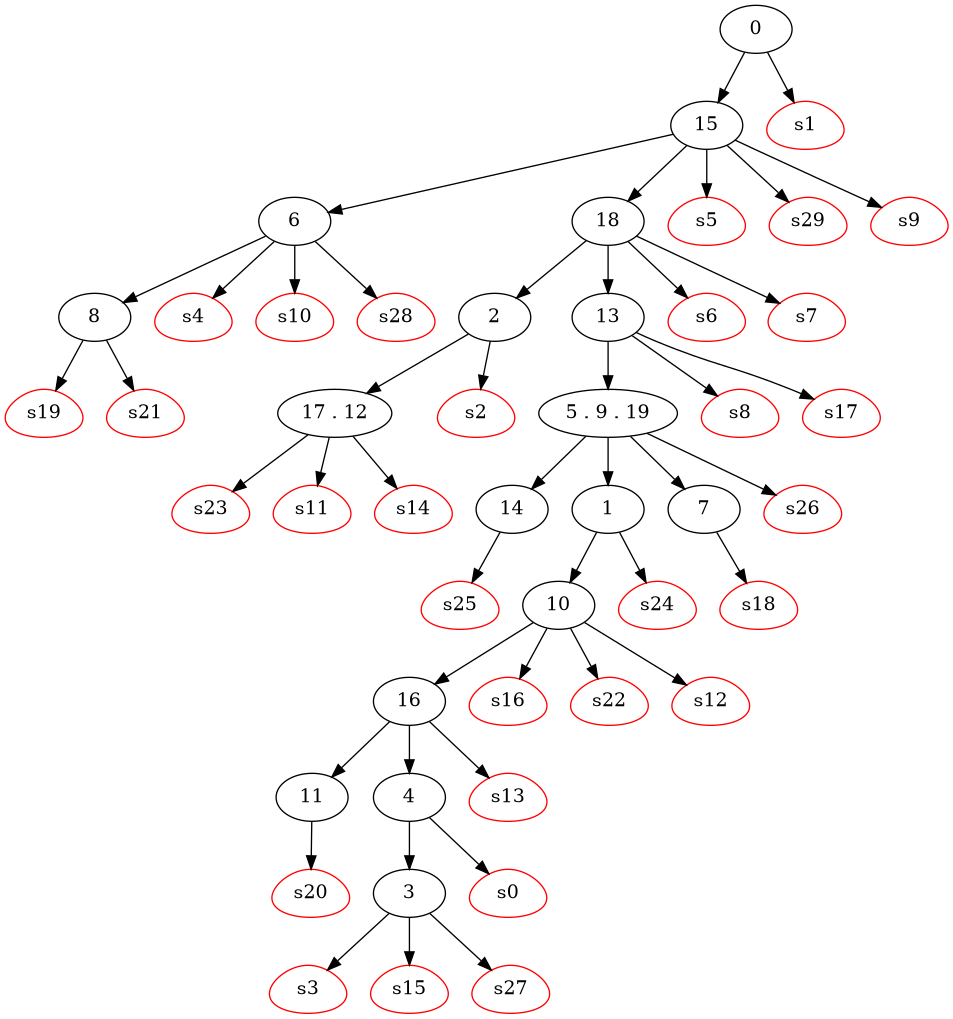
\includegraphics[width=0.62\textwidth]{img/dataset/s/treeF_zeta=1_gamma=0.15_alpha=0.01_beta=0.1_MR=0.02_N=30_M=20.png}
	\caption{درخت جهش تصادفی با پارامتر‌های $N=30, M=20, \zeta=1, \gamma=0.15$}
	\label{fig:mtn30m20z1g0.15}
\end{figure}

\subsubsection{تبدیل درخت به ماتریس ژن-سلول}
با داشتن درخت (تولید شده با هرکدام از روش‌ها تفاوتی ندارد) در ادامه ابتدا از روش مدل‌سازی \glspl{infinitesites} ماتریس را تشکیل می‌دهیم و پس از آن فرض حذف برخی از جهش‌ها را در آن مشابه با مقاله \lr{scarlet} اضافه می‌کنیم و پروفایل‌های تغییر تعداد کپی را به عنوان داده‌های تکمیلی برای درخت و داده‌های \gls{snv} می‌سازیم.
%\vspace{20pt}
\\
\noindent\textbf{فرض مدل مکان‌های بی‌نهایت}\LTRfootnote{Infinite Sites Model}\\
در این حالت فرض می‌کنیم که هر جهش اتفاق افتاده در درخت فیلوژنی در تمامی نسل‌های پس از آن باقی می‌ماند و هیچ‌گاه از بین نمی‌رود. در چنین حالتی درخت حاصل از این روش درختی یکتا بوده که به نام درخت فیلوژنی کامل\LTRfootnote{Perfect Phylogeny Tree} شناخته می‌شود.
\\
در این قسمت باید با استفاده از درخت تصادفی تولید بتوانیم ماتریس جهش‌ها را برای سلول‌های مختلف با فرض مکان‌های بی‌نهایت بدست آوریم. 
در ابتدا ماتریس $E$ را به ابعاد $M\times N$ ایجاد می‌کنیم و برای هر درایه $i,j$ در آن که $i$ شماره جهش و $j$ شماره سلول است به صورت فرمولی که در ادامه آمده است مقداردهی می‌کنیم.
\begin{equation}
	E_{i,j} = 
	\begin{cases} 
		1  \quad &\text{\lr{if}} \quad \text{\lr{mutation }} i \text{\lr{ is an ancestor of cell }} j \\
		0 \quad &\text{\lr{o.w}}
	\end{cases}
\end{equation}
به این ترتیب با فرض مدل مکان‌های بی‌نهایت ماتریس بدون خطا $E$ را داریم که در گام بعد آن‌ها ممکن است این فرض برایشان نقض شود و جهش‌هایی پس از وقوع حذف شوند.

\subsubsection{تولید پروفایل‌های تعداد کپی و تعیین جهش‌های مسافر}
پس از ساخت درخت و تبدیل آن به ماتریس $E$ طبق فرض مدل مکان‌های بی‌نهایت، حال با توجه به مقدار پارامترهای $\psi$، $\vartheta$ و $\varrho$ به تغییر در ساختار ماتریس $E$ و ساخت داده‌های پروفایل تعداد کپی می‌پردازیم.
پارامتر $\psi$ تعیین ‌کننده احتمال فقدان یک جهش، پارامتر $\vartheta$ میزان تاثیر در وقوع فقدان متناسب با فاصله از وقوع جهش و پارامتر $\varrho$ احتمال کاهش تعداد کپی بدون از دست رفتن جهش را کنترل می‌کنند.
\\
حال که درخت را داریم کافی است تا برگ‌ها را کنار بگذاریم و از بین نود‌های باقی مانده در درخت $T$، با احتمال مشخص شده $\psi$ جهش‌ها را برای حذف انتخاب ‌کنیم. دلیل کنار گذاشته شدن برگ‌ها نیز مشخص است زیرا که اگر آن‌ها قرار باشد حذف شوند چون برگ هستند دیگر زیر درختی ندارند که بخواهند حذف خود را در آن‌جا رقم بزنند. پس در نتیجه دقت شود که از روی این پارامتر تعداد جهش‌های حذف‌شونده را نمی‌توان حدس زد و تعداد آن‌ها به چاقی یا لاغری درخت بستگی دارد بطوریکه هرچه درخت لاغرتر باشد در آن صورت این احتمال به تعداد حذف شده‌ها نزدیکتر خواهد بود و بلاعکس.\\
پس از مشخص شدن جهش‌های حذف‌شونده حال زیردرخت‌های آن‌ها را جدا می‌کنیم و متناسب با پارامتر $\vartheta$ یکی از نودهای نوادگان را به عنوان محل فقدان انتخاب می‌کنیم. این عمل طبق رابطه \ref{eq:ch_er:loss_loc} انجام می‌شود.
\begin{equation}
	P_l(x|i) = \vartheta e^{-\vartheta *\text{\lr{dist($x$,$i$)}}}
	\label{eq:ch_er:loss_loc}
\end{equation}
این رابطه همان توزیع نمایی است که برای فضای پیوسته تعریف شده است. ما فاصله نودهای زیردرخت ($x$) را به جهش انتخاب شده $i$ در زیر درخت آن ژن در نظر می‌گیریم و متناسب با این رابطه و احتمال یکی از آن‌ها را به عنوان محل فقدان انتخاب می‌کنیم. مشخص است که هر چه این مقدار پارامتر کوچکتر باشد این انتخاب محل فقدان به فاصله تا ژن انتخابی کمتر تاثیرگذار می‌شود.
\\
در نهایت پس از این مرحله نوبت به تولید پروفایل‌های تعداد تکرار برای نمونه‌ها می‌رسد. ما بردار پروفایل تکرار را $k$ واحد درنظر می‌گیریم و ژن‌ها را در بین آن‌ها توزیع می‌کنیم. در این پایگاه داده تمرکز ما در تولید این پروفایل‌ها به مقادیر کپی‌ها نیست بلکه به نحوه تغییر آنهاست که افزایشی است یا کاهشی. بنابرین با یک مقدار اولیه تصادفی نمونه‌های اولیه که به ریشه متصل شده‌اند را مقداردهی می‌کنیم و در ادامه با توجه به اینکه محل اتصال نمونه‌ها کجاست آن‌ها را بدون تغییر باقی میگذاریم یا فقط افزایش می‌دهیم. پس از این کار ژن‌های انتخاب شده برای حذف را به همراه درصدی که پارامتر $\varrho$ مشخص می‌کند را درون یک لیست می‌گذاریم و تمام نمونه‌های مرتبط با آن‌ها را به صورت تصادفی بین $1$ تا $3$ واحد کاهش می‌دهیم تا پروفایل‌های $C$ برای نمونه‌ها ساخته شود.\\
مشخص است که این عملیات هیچ تغییری در ساختار درخت ایجاد نمی‌کند و صرفا کافی است در کنار داده‌های ساخته شده ‌$C$، در درخت، نودهای حذف شونده و محل حذف آن‌ها را مشخص کنیم تا آماده ورود به مرحله بعد که ساخت ماتریس از روی این درخت است برویم.
\\
در نهایت خروجی این بخش برای تصاویر درختان تولید شده قبل در شکل \ref{fig:E} قابل مشاهده می‌باشند. 
\begin{figure}[!ht]
	\centering
	\subfloat[ماتریس درخت شکل \ref{fig:dstn20zeta1}]{
		\centering
		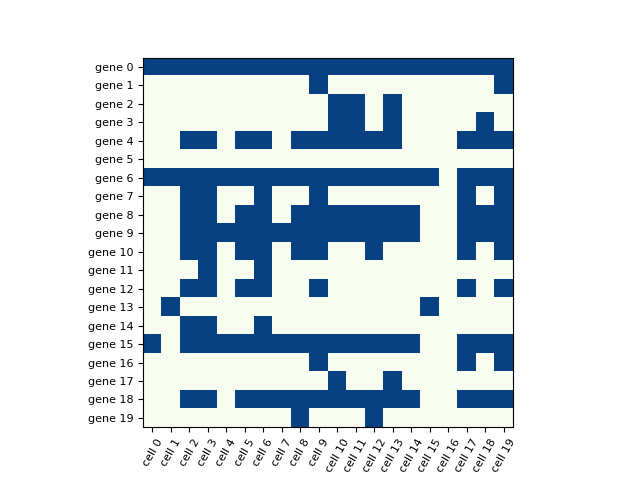
\includegraphics[width=0.55\textwidth]{img/dataset/s/zeta1n20m20}
		\label{fig:Edstn20zeta1}
	}
	\hfill
	\subfloat[ماتریس درخت شکل \ref{fig:mtn30m20z1g0.15}]{
		\centering 
		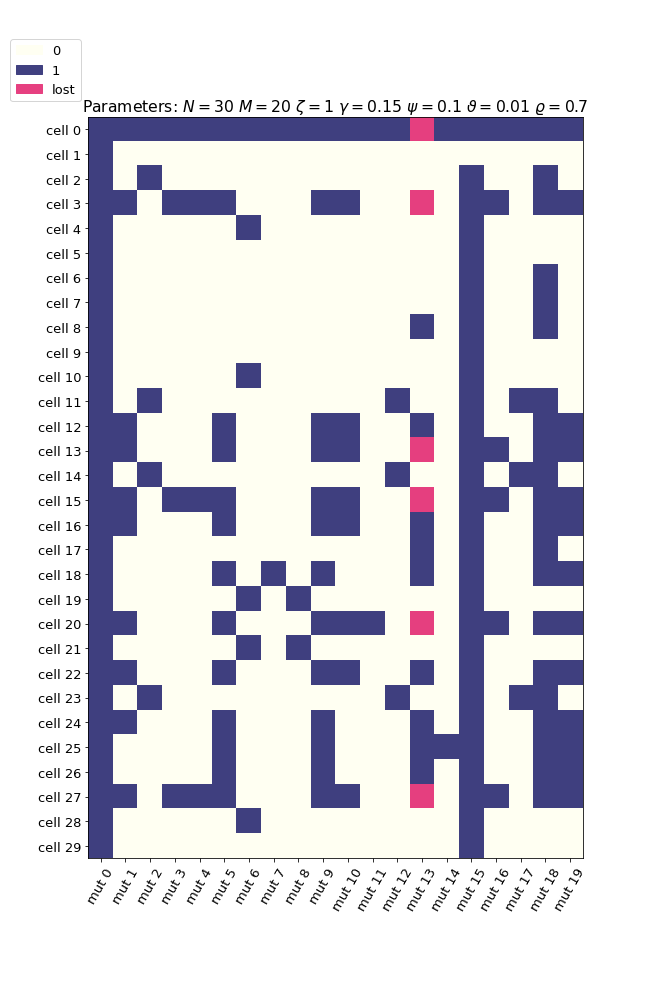
\includegraphics[width=0.42\textwidth]{img/dataset/s/El_zeta=1_gamma=0.15_alpha=0.01_beta=0.1_MR=0.02_N=30_M=20.png}
		\label{fig:E_mt_N30_M20_Z1_G0.15}
	}
	\caption{ماتریس‌های ژن-سلول ($E$) بدست آمده از درخت‌های تصادفی ساخته شده}
	\label{fig:E}
\end{figure}
همانطور که مشخص است برای یکی از درختان فقدان یک جهش بوجود آمده است و برای دیگری نه. 
\subsubsection{اضافه کردن نویز به ماتریس ژن-جهش}
برای قسمت نهایی آماده‌سازی پایگاه داده مجازی نیاز است تا به ماتریس $E$ با پارامتر $\Theta=(\alpha, \beta, m_r)$ نویز اضافه کنیم و آن را به ماتریس $D$ تبدیل کنیم که $\alpha=P(D_{ij}=1|E_{ij}=0)$ و $\beta=P(D_{ij}|E_{ij})$ است و همچنین $m_r\in(0,1)$ که نرخ داده‌های از دست رفته را مشخص می‌کند.
\\
برای این منظور به ازای تمامی درایه‌های $0$ ماتریس $E$ هربار یک عدد تصادفی با توزیع یکنواخت بین $[0,1)$ بوجود می‌آوریم و اگر عدد تولید شده کوچکتر از $\alpha$ بود آنگاه ان درایه در ماتریس $D$ را برابر با $1$ قرار می‌دهیم. به همین ترتیب مجددا این بار برای درایه‌های $1$ ماتریس $E$ این‌کار را تکرار می‌کنیم و اگر عدد تصادفی تولید شده کوچکتر از $\beta$ شد، درایه متناظر را در ماتریس $D$ برابر با $0$ قرار می‌دهیم.
\\
پس از اتمام کار نوبت به اضافه کردن داده‌های از دست رفته است. برای این منظور با نرخ $m_r$ بعضی از درایه‌های ماتریس $D$ را برابر با $2$ قرار می‌دهیم که به منزله در دسترس نبودن اطلاعات است. نام ماتریس نهایی را که شامل داده‌های از دست رفته است $D_m$ می‌گزاریم. در ادامه تصاویر اضافه شدن نویز به ماتریس شکل \ref{fig:E_mt_N30_M20_Z1_G0.15} در شکل \ref{fig:D} آمده است.
\begin{figure}[!ht]
	\subfloat[ماتریس نویزی با $\alpha=0.01, \beta=0.1$]{
		\centering
		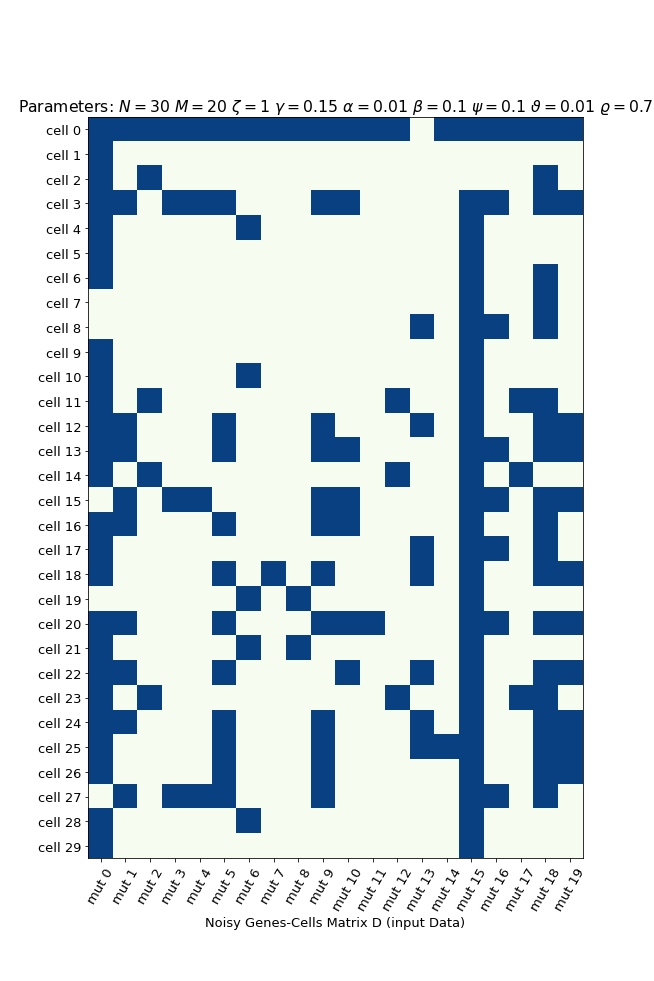
\includegraphics[width=0.32\textwidth]{img/dataset/s/D_zeta=1_gamma=0.15_alpha=0.01_beta=0.1_MR=0.02_N=30_M=20.png}
		\label{fig:D_mt_N30_M20_Z1_G0.15}
	}
	\hfill
	\subfloat[نویزی اضافه شده با پارمترهای $\alpha=0.01, \beta=0.1$]{
		\centering 
		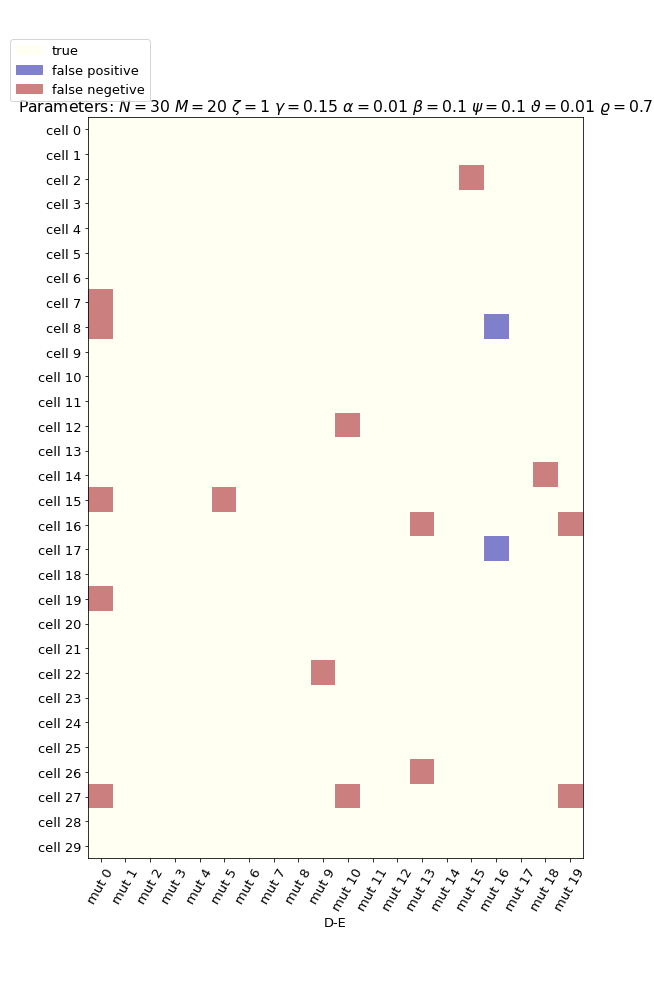
\includegraphics[width=0.32\textwidth]{img/dataset/s/DmE_zeta=1_gamma=0.15_alpha=0.01_beta=0.1_MR=0.02_N=30_M=20.png}
		\label{fig:DmN_mt_N30_M20_Z1_G0.15}
	}
%	\vskip\baselineskip
%	\centering
	\hfill
	\subfloat[ماتریس نویزی به همراه داده‌های از دست رفته با پارامترهای $\alpha=0.1, \beta=0.08, m_r=0.1$]{
		\centering 
		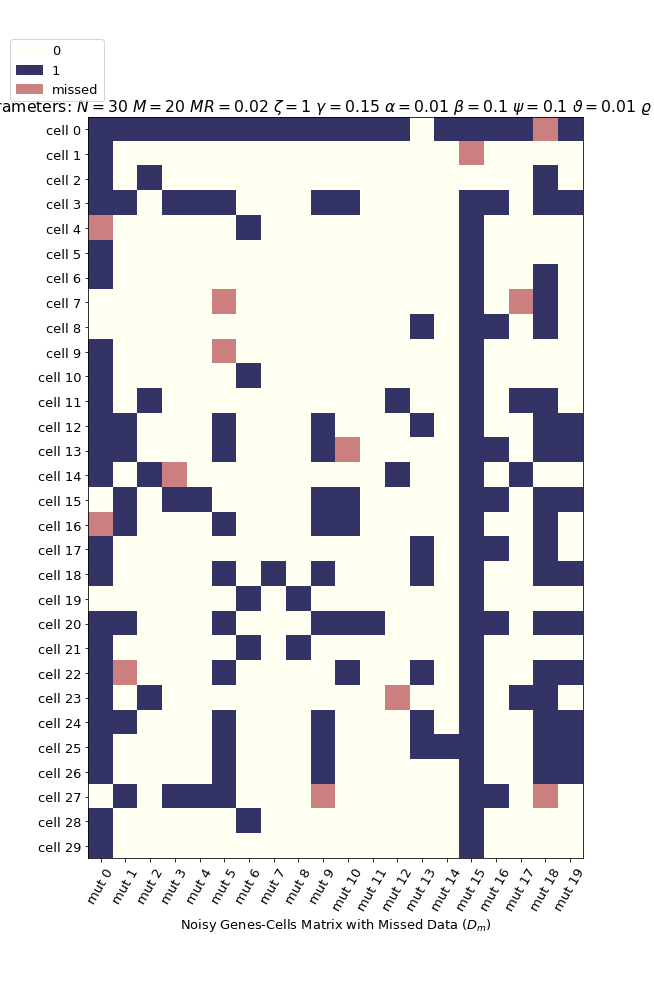
\includegraphics[width=.32\textwidth]{img/dataset/s/Dm_zeta=1_gamma=0.15_alpha=0.01_beta=0.1_MR=0.02_N=30_M=20.png}
		\label{fig:Dm_mt_N30_M20_Z1_G0.15}
	}
	\caption{ماتریس‌های ژن-سلول همراه با نویز و داده‌های از دست رفته شکل \ref{fig:E_mt_N30_M20_Z1_G0.15} که برای ورودی مسله آماده شده است.}
	\label{fig:D}
\end{figure}


\subsection[پایگاه داده حقیقی]
{پایگاه داده حقیقی
	\LTRfootnote{Real Dataset}
}
به عنوان پایگاه داده حقیقی از پایگاه داده استفاده شده در مقاله \lr{SCITE} به عنوان پایگاه داده حقیقی اصلی استفاده خواهیم کرد \cite{davis2016computing}.

%که ماتریس داده ورودی آن به صورت شکل  \ref{fig:navin_Dm} می‌باشد.
%\begin{figure}[!ht]
%	\centering 
%	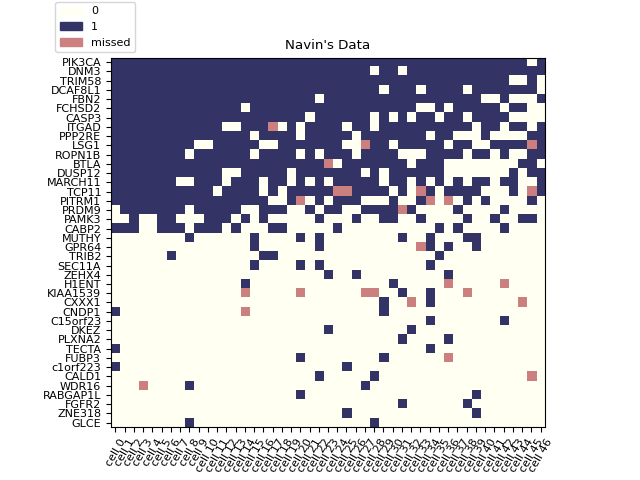
\includegraphics[width=0.67\textwidth]{img/dataset/r/Navin_Dm.png}
%	\caption{داده‌های حقیقی \lr{Navin} در مقاله \lr{SCITE}}    
%	\label{fig:navin_Dm}
%\end{figure}

%همچنین پایگاه‌داده حقیقی \lr{Xu} نیز که در مقاله \lr{SCITE} مورد استفاده قرار گرفته است در شکل \ref{fig:Xu_Dm} آمده است.
%\begin{figure}[!ht]
%	\centering 
%	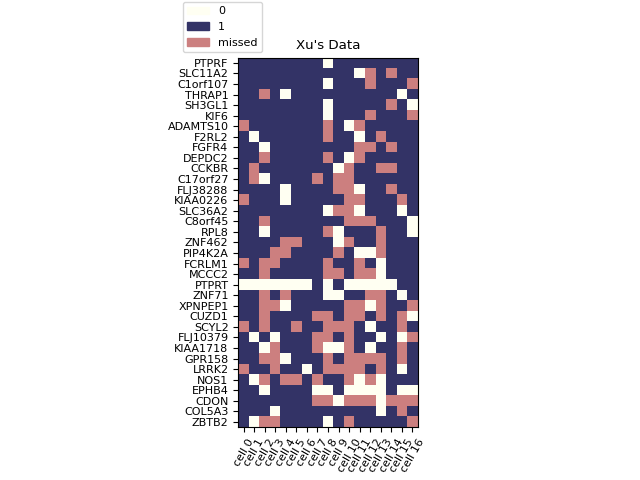
\includegraphics[width=0.625\textwidth]{img/dataset/r/Xu_Dm.png}
%	\caption{داده‌های حقیقی \lr{Xu} در مقاله \lr{SCITE}}    
%	\label{fig:Xu_Dm}
%\end{figure} 

\subsection{آموزش شبکه }
پس از ساخت پایگاه داده مجازی حال می‌توان به آموزش شبکه معرفی شده در \ref{sec:ch_pm:network} پرداخت.
\\
به شکل \ref{fig:ch_er:td3} توجه کنید.
\begin{figure}[!ht]
	\centering 
	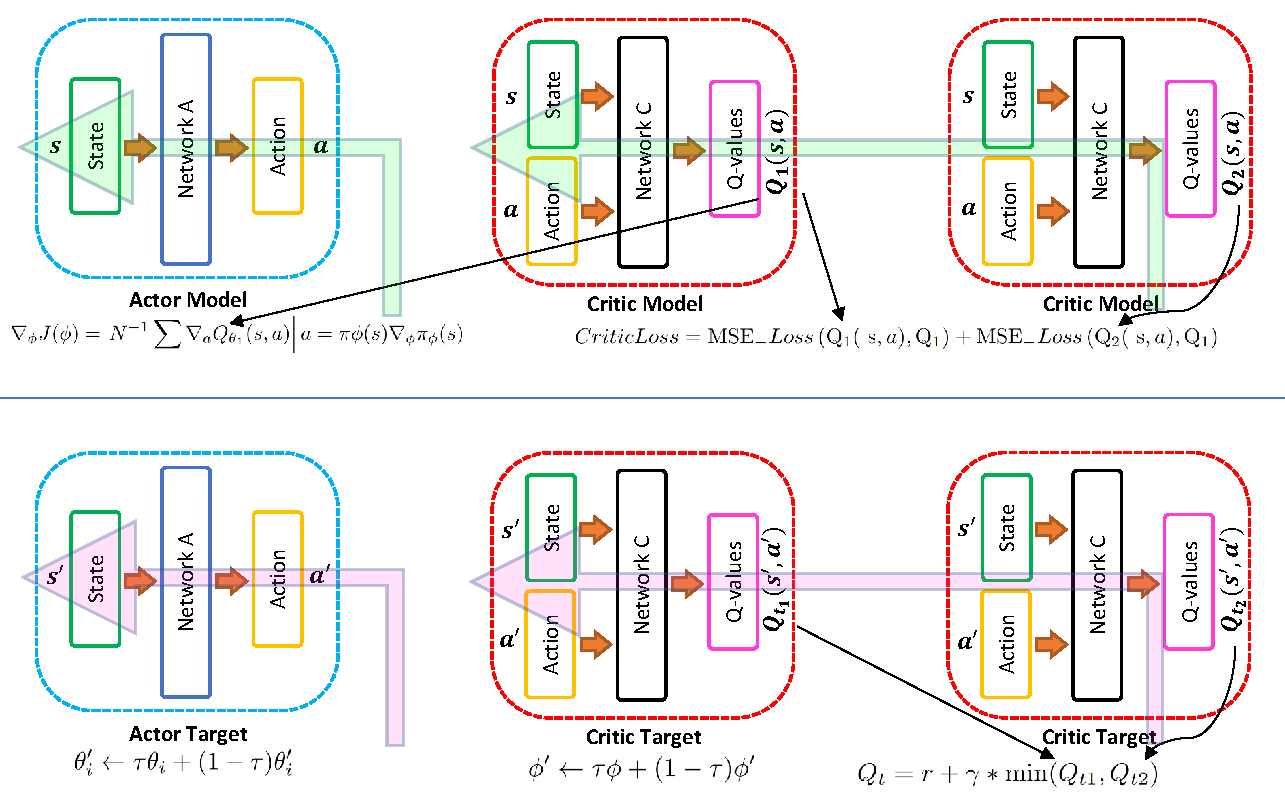
\includegraphics[width=\textwidth]{img/chaps/er/td3_crop}
	\caption{نحوه آموزش شبکه با استفاده از ساختار \lr{TD3} \cite{fujimoto2018addressing}.}    
	\label{fig:ch_er:td3}
\end{figure} 

شکل \ref{fig:ch_er:td3} متد ارائه شده در \cite{fujimoto2018addressing} را نمایش می‌دهد که شامل ۱۵ مرحله برای آموزش است که شبکه پیشنهادی خود را به این فرم آموزش دادیم. این مراحل به شرح زیر می‌باشد.
\begin{enumerate}
	\item
ما یک حافظه ۵۰ هزارتایی به عنوان حافظه‌ای از تجربیات انتخاب عمل‌های مختلف\LTRfootnote{Experience replay memory} را در نظر می‌گیریم که در هر انتقال (تکرار) آن را مقداردهی خواهیم کرد.
\item
ساخت یک شبکه برای عملگر مدل (\lr{actor model}) و یک شبکه برای عملگر هدف (\lr{actor target})
\item
ساخت دو شبکه برای نقاد مدل (\lr{critic model}) و دو شبکه برای نقاد هدف (\lr{critic target})
	
\item
در این مرحله یک دسته از انتقال‌های ($s, s', a, r$) را از حافظه انتخاب می‌کنیم. سپس برای هر نمونه از این دسته موارد بعدی را انجام می‌دهیم.
\item
از شرایط حالت بعدی $s'$، عملگر هدف عملیات $a'$ را انجام خواهد داد.
\item
ما یک نویز گوسی (نرمال) به این عملیات بعدی $a'$ اضافه خواهیم کرد و البته نمی‌گذاریم نتیجه حاصله خارج از محدوده قابل قبول قرار بگیرد.
\item
دو شبکه نقاد هدف مقادیر ($s',a'$) را به عنوان ورودی دریافت می‌کنند و در خروجی مقادیر
 \lr{Q-values}، 
$Q_{t1}(s',a')$
 و
 $Q_{t2}(s',a')$
  را تولید می‌کنند.
\item
ما کوچکترین مقدار \lr{Q-values} تولید شده را برمی‌گزینیم: $\min(Q_{t1}, Q_{t2})$. این مقدار در واقع ارزش حالت بعد را تخمین می‌زند.
\item
ما مقدار
$$Q_t=r+\gamma\min(Q_{t1}, Q_{t2})$$
 را از خروجی شبکه‌های نقاد هدف محاسبه می‌کنیم
\item
دو شبکه نقاد مدل مقدار ($s,a$) را دریافت می‌کنند و خروجی‌های 
$Q_1(s,a)$ و $Q_2(s,a)$
 را تولید می‌کنند.
\item
ما مقدار خطا را برای شبکه‌های نقاد مدل به صورت
$$\text{\lr{critic loss = MSE($Q_1, Q_t$)+MSE($Q_2, Q_t$)}}$$
 محاسبه می‌کنیم.
\item
خطای محاسبه شده را برای شبکه‌های نقاد مدل با یک بهینه‌ساز \lr{SDG}، \gls{backpropagate} می‌کنیم
\item
در هر 2 \gls{iteration} یک‌بار، شبکه عملگر مدل را با استفاده از \lr{gradient ascent} بر روی خروجی حاصل از شبکه نقاد مدل اول به صورت
$$\nabla_{\phi}J(\phi)=N^{-1}\Sigma\nabla_aQ_{\theta_1}(s,a)|_{a=\pi_\phi(s)}\nabla_\phi\pi_\phi(s)$$
به روزرسانی می‌کنیم. جایی که $\phi$ و $\theta_1$ به وزن‌های شبکه عملگر و نقاد اشاره می‌کند.
\item
در هر 2 \gls{iteration} یک‌بار، ما وزن‌های شبکه عملگر هدف را به روش \gls{polyakaveraging} به صورت 
$$\theta'_i \leftarrow \tau\theta_i+(1-\tau)\theta'_i$$
به روزرسانی می‌کنیم.
\item
در هر 2 \gls{iteration} یک‌بار، ما وزن‌های شبکه نقاد هدف را به روش \gls{polyakaveraging} به صورت 
$$\phi'_i \leftarrow \tau\phi_i+(1-\tau)\phi'_i$$
 به روزرسانی می‌کنیم.
\end{enumerate}
برای آموزش با توجه نتایجی که در \cite{azer2020tumor} بدست آمده است، یک مرحله پیش‌پردازش را که در آن ماتریس ورودی طبق روش \cite{gusfield1997algorithms} مرتب‌سازی می‌شود را انتخاب می‌کنیم و در ادامه نتایج گزارش‌شده همگی با این پیش‌پردازش خواهند بود.
\\
در ادامه در شکل \ref{fig:ch_er:td3_learning} نتایج آموزش شبکه برای ماتریس‌های با سایز ورودی $15\times 12$ قابل مشاهده است.
\begin{figure}[!ht]
	\subfloat[پارامترهای حذف جهش $\psi=0.1, \vartheta=0.01, \varrho=0.7$]{
		\centering
		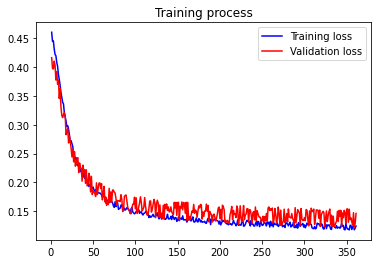
\includegraphics[width=0.48\textwidth]{img/chaps/er/net_loss}
		\label{fig:D_mt_N30_M20_Z1_G0.15}
	}
	\hfill
	\subfloat[پارامترهای خطا برابر با $\alpha=0.003, \beta=0.05$]{
		\centering 
		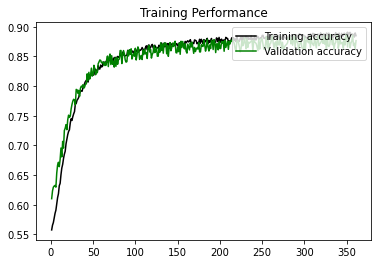
\includegraphics[width=0.48\textwidth]{img/chaps/er/net_acc}
		\label{fig:DmN_mt_N30_M20_Z1_G0.15}
	}
%		\vskip\baselineskip
%		\centering
%%	\hfill
%	\subfloat[ماتریس نویزی به همراه داده‌های از دست رفته با پارامترهای $\alpha=0.1, \beta=0.08, m_r=0.1$]{
%		\centering 
%		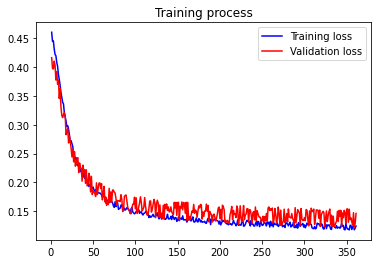
\includegraphics[width=.48\textwidth]{img/chaps/er/net_loss}
%		\label{fig:Dm_mt_N30_M20_Z1_G0.15}
%	}
%	\hfill
%	\subfloat[ماتریس نویزی به همراه داده‌های از دست رفته با پارامترهای $\alpha=0.1, \beta=0.08, m_r=0.1$]{
%		\centering 
%		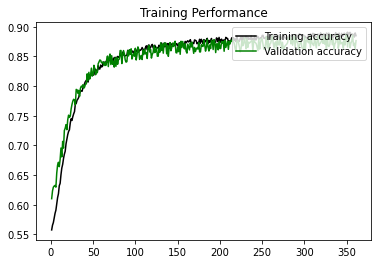
\includegraphics[width=.48\textwidth]{img/chaps/er/net_acc}
%		\label{fig:Dm_mt_N30_M20_Z1_G0.15}
%	}
	\caption{نتیجه آموزش شبکه برای ماتریس‌های ورودی با ابعاد $15\times 12$.}
	\label{fig:ch_er:td3_learning}
\end{figure}



\newpage
\section{نتایج تجربی}
در این بخش به نتایج بدست آمده برای روش پیشنهادی می‌پردازیم و برای هر دو داده مصنوعی و حقیقی نتایج بدست آمده را نمایش خواهیم داد.
\subsection{نتایج بر روی پایگاه داده مصنوعی}
همان‌گونه که در بخش دوم توضیح داده شد با توجه به سختی دسترسی به پایگاه داده‌های حقیقی و اینکه در آن‌ها نیز حقیقت داده‌ها ($E$) وجود ندارد تصمیم به ایجاد پایگاه داده‌ای مصنوعی گرفته شد که با کمک آن بتوان ارزیابی مناسبی از روش پیشنهادی و میزان کارایی و مقاومت روش را نسبت به تغییر پارامترها سنجید.

فرض کنید ماتریس ورودی شکل \ref{fig:sy_D1} را در اختیار داریم و می‌خواهیم بهترین درخت فیلوژنی را برای آن بیابیم.
\begin{figure}[!ht]
	\centering
	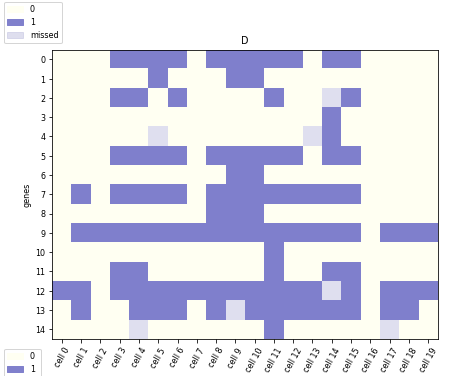
\includegraphics[width=0.65\textwidth]{img/chaps/er/s_input_D}
	\caption{نمونه‌ای تصادفی از ماتریس ورودی $D$}
	\label{fig:sy_D1}
\end{figure}

حال یک درخت تصادفی به صورت شکل \ref{fig:sy_initial_T1} می‌سازیم.
\begin{figure}[!ht]
	\centering
	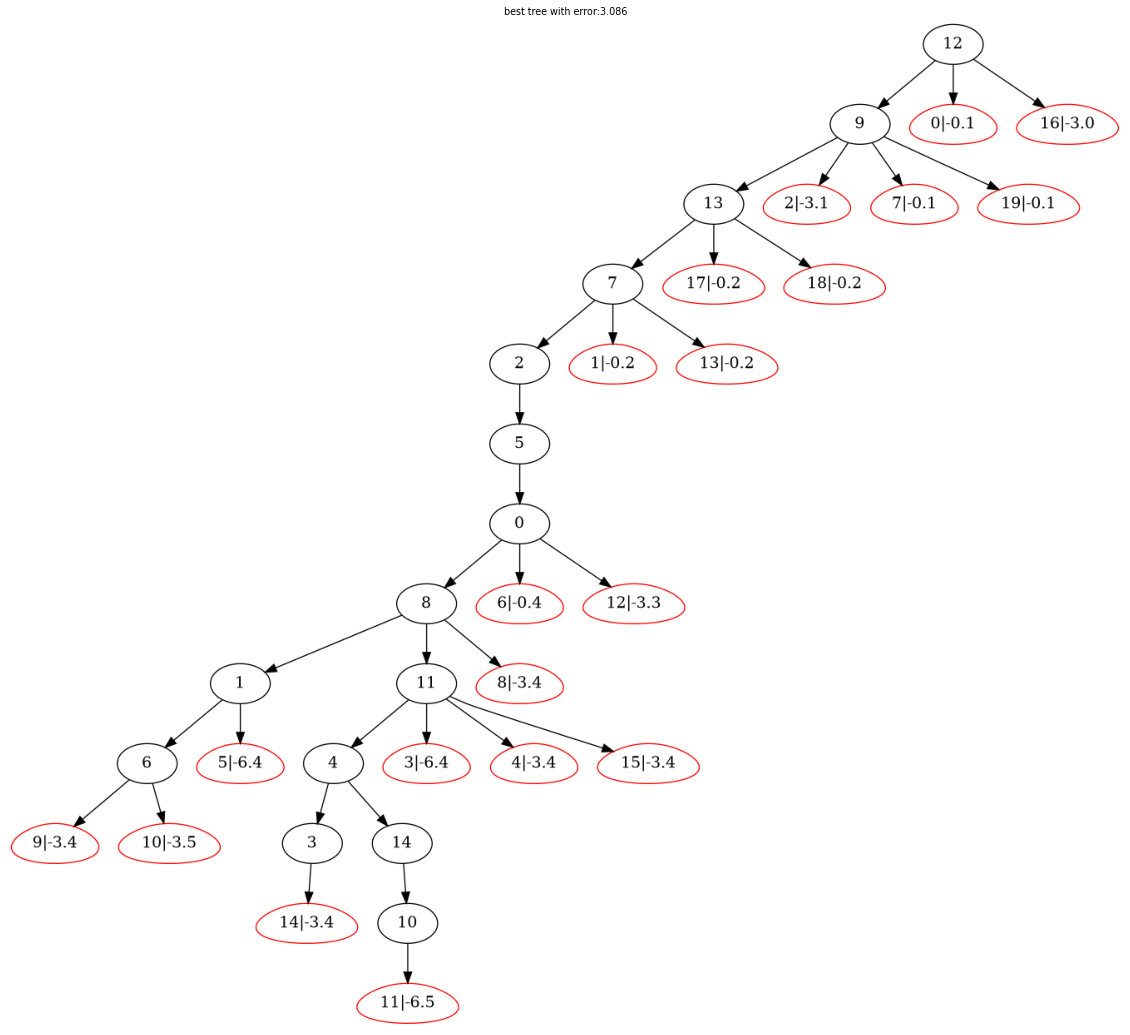
\includegraphics[width=0.8\textwidth]{img/chaps/er/initial_s_tree}
	\caption{‌درخت تصادفی ایجاد شده به عنوان درخت اولیه شکل \ref*{fig:sy_D1}}
	\label{fig:sy_initial_T1}
\end{figure}
در درخت شکل  \ref{fig:sy_initial_T1} نمونه‌ها (سلول‌ها) با رنگ قرمز به درخت متصل شده‌اند که البته این ضمیمه بهترین ضمیمه ممکن است و ضریبی از میزان خطای هر ضمیمه نیز در کادر قرمز رنگ سلول‌ها به صورتی عددی منفی نوشته شده است. 
\\
برای مشاهده خروجی روش پیشنهادی و مقایسه آن با حالت پایه می‌توان نتیجه حاصله برای ماتریس ورودی \ref{fig:sy_D1} را در شکل \ref{fig:sy_benchmark1} مشاهده کرد.



در این شکل دو درخت وجود دارد که درخت سمت راستی درخت حقیقی است که به دنبال آن بودیم و درخت سمت چپ بهترین درخت یافته شده است. همچنین در پایین شکل، ۹ ماتریس مشاهده می‌شود که ماتریس‌ها سمت راست و پایین به نوعی بیان‌کننده میزان خطا بین ۴ ماتریس سمت چپ بالا می‌باشند. در بالای هر ماتریس نام آن نوشته شده است و در نهایت در انتهای تصویر نیز روند کاهش خطا و تلاش‌های روش پایه ما که \lr{SCITE} می‌باشد در گام‌های مختلف قابل مشاهده است. فقط نکته‌ای که وجود دارد این است که خطای نوشته شده در تصاویر برابر ضریبی از خطای اصلی می‌باشد و خود آن نیست.
\\
همان‌گونه که مشخص است در ماتریس $D$ هفت داده از دست رفته وجود دارد که چهار تا از آن‌ها در حقیقت جهش یافته و بقیه خیر. اگر ما در محاسبات خود این هفت داده را در محاسبه خطا در نظر نگیریم و با تغییر ۶ داده دیگر می‌توانیم به ماتریس $\hat{E}$ (در شکل به نام $E$ نوشته شده است) برسیم که معادل بهترین درخت بدست آمده است. که این یعنی ماتریس $D$ ما با بیش از ۴۰ تغییر بدست ما رسیده است. حال اگر حقیقت داده‌ها و درخت اصلی را مشاهده کنیم می‌بینیم که در آنجا فقط ۶ خطا وارد شده است که فقط ۴ مورد از آن‌ها درست کشف شده است و در عوض تعداد بسیار زیادی از داده‌ها را خراب کرده است. بنابرین الگوریتم بدون اطلاع از حقیقت توانسته با  ۴۵ خطا به یک درخت فیلوژنی مناسب دست بیابد. بنابرین روش پایه توانسته درخت فیلوژنی را با صحت 
${15*20 - 45\over15*20} = 0.85\overline{3}$
بازسازی کند که عددی جالبی با توجه به $5000$ تکرار نمی‌باشد.
\begin{figure}[!ht]
	\centering
	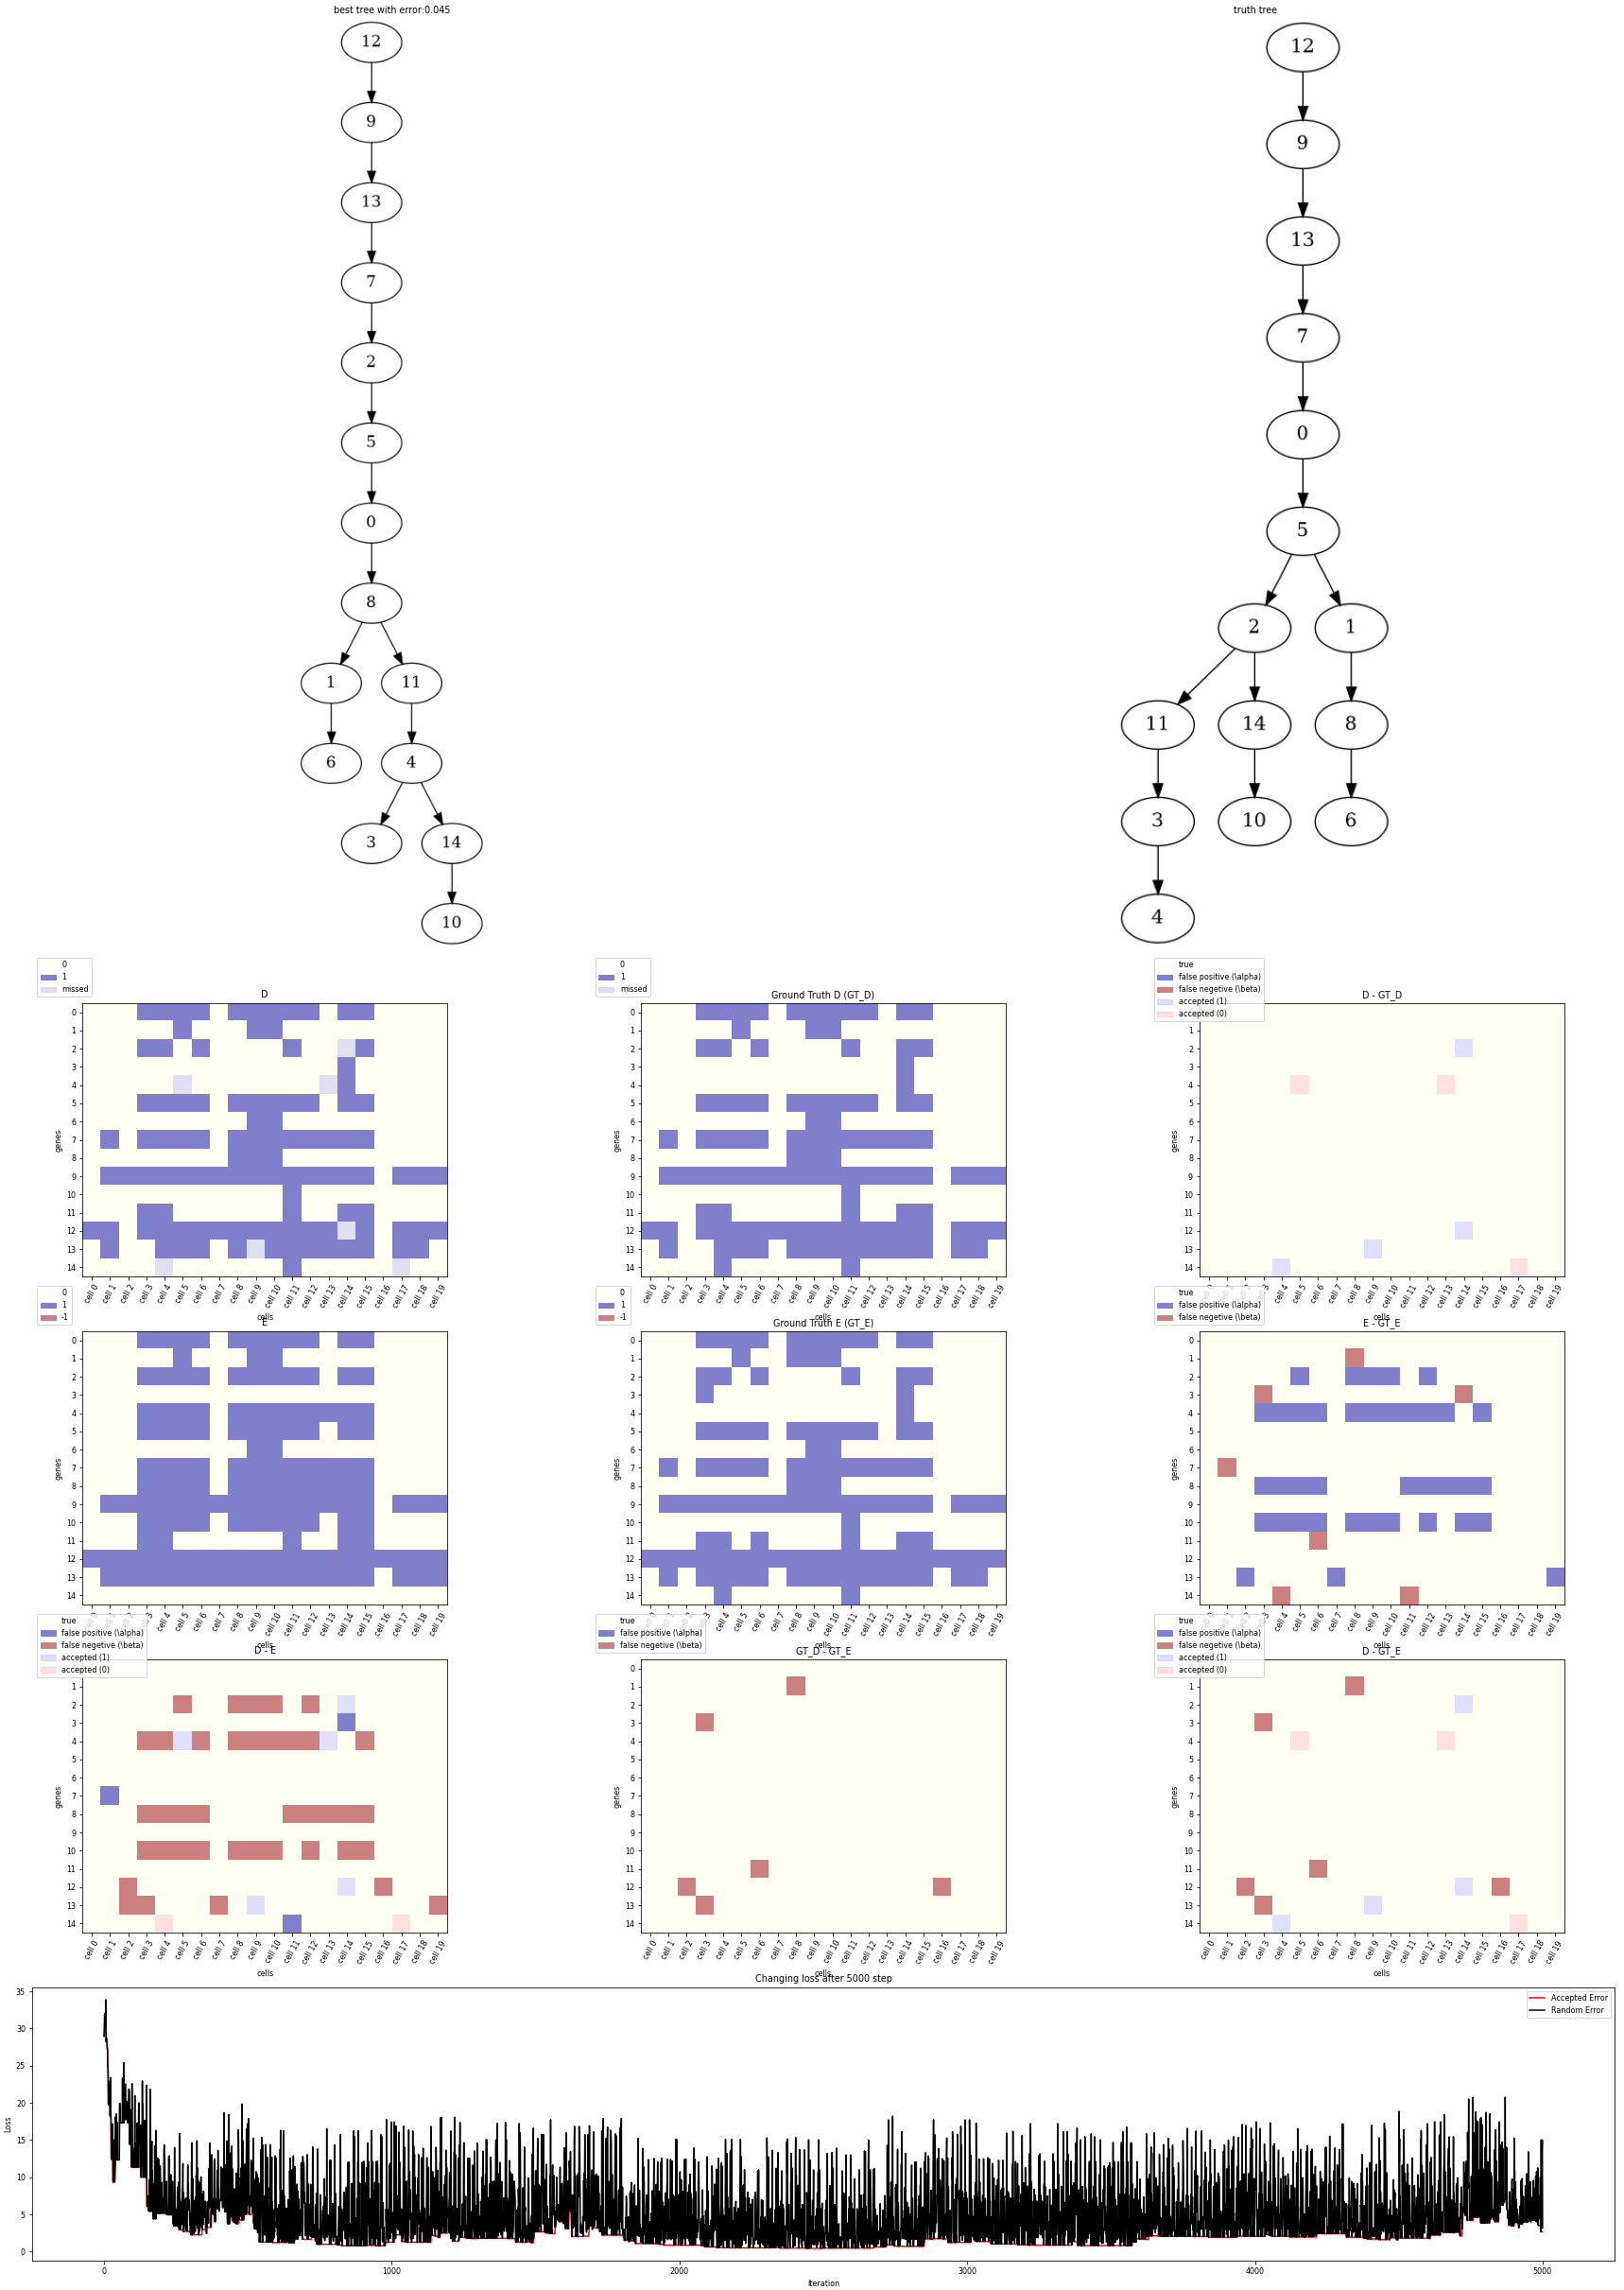
\includegraphics[height=0.9\textheight]{img/chaps/er/SCITE_s_tree}
	\caption{‌نتیجه استنتاج درخت فیلوژنی با روش پایه مشابه به مقاله scite برای ماتریس شکل \ref*{fig:sy_D1}}
	\label{fig:sy_benchmark1}
\end{figure}

اما نتیجه روش پیشنهادی خود بر روی همین داده ورودی در شکل \ref{fig:sy_benchmark_pm} قابل مشاهده است. حال اگر به پاسخی که روش ارائه شده برای این ورودی بدست آورده است را دقت کنیم متوجه خواهیم شد که بازسازی نسبت به حالت قبل با دقت بالاتری انجام شده است که هم به صورت چشمی با مقایسه درخت و هم به صورت محاسبه تعداد بازسازی‌های درست که برابر با 
${15*20 - 5\over15*20} = 0.98\overline{3}$
می‌شود، که نشان دهنده مطلوبیت و قدرت روش پیشنهادی است. مخصوصا اگر شکل \ref{fig:sy_benchmark_pm_chart} را مشاهده نمایید و متوجه شوید که برخلاف روش پایه این استنتاج تنها با استفاده از $377$ تکرار انجام شده که دلیل آن همان استفاده از یک شبکه با انتخاب‌های هوشمند در کنار فرض حذف جهش‌های مسافر است. البته باید اذعان کنیم که هر تکرار ما بخاطر بهینه‌سازی‌ای که به ازای هر درخت دارد چندین برابر زمان هر اجرای روش پایه می‌باشد که در قسمت‌های بعدی بیشتر در خصوص این موارد صحبت خواهیم نمود.

\begin{figure}[!ht]
	\centering
	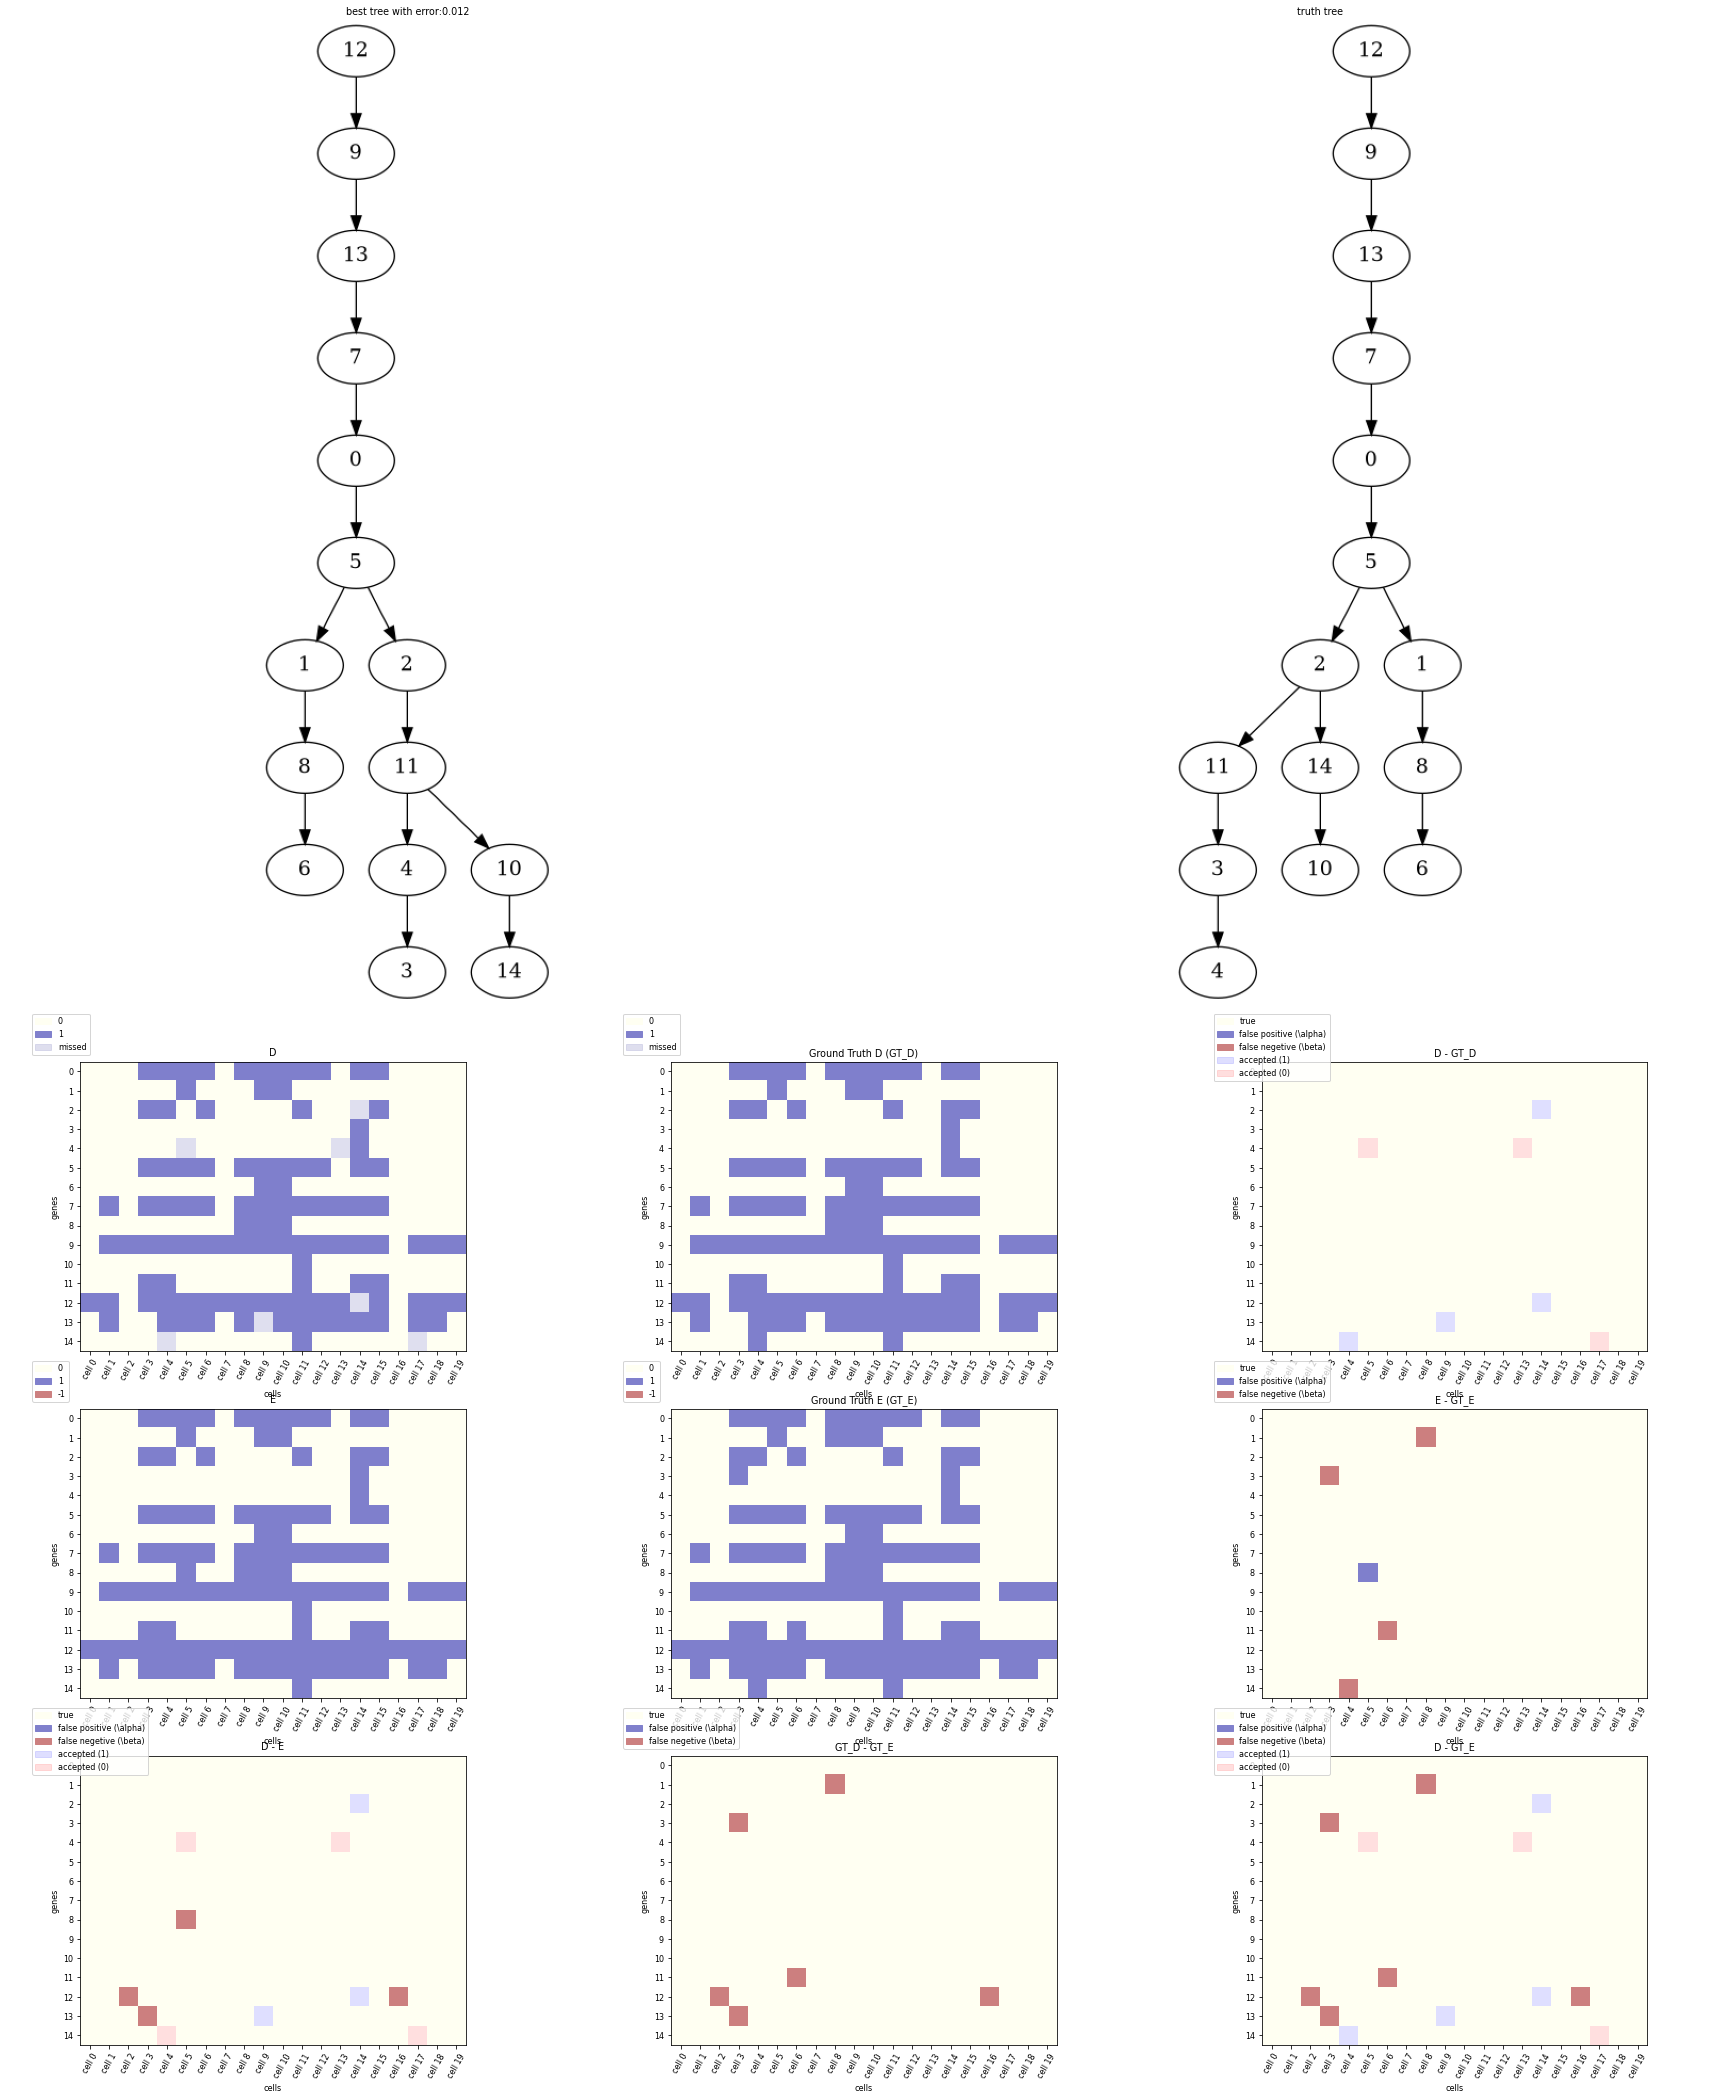
\includegraphics[height=0.85\textheight]{img/chaps/er/PM_s_tree}
	\caption{‌نتیجه استنتاج درخت فیلوژنی با روش پیشنهادی ارائه شده برای ماتریس شکل \ref*{fig:sy_D1}}
	\label{fig:sy_benchmark_pm}
\end{figure}

\begin{figure}[!ht]
\centering
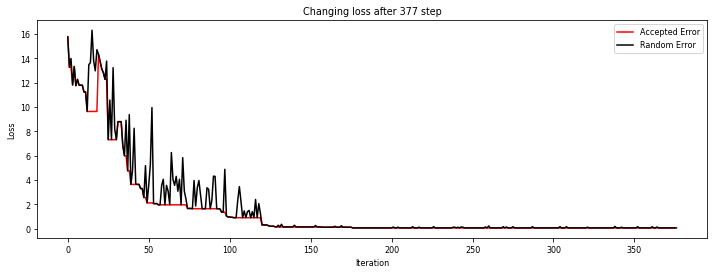
\includegraphics[height=0.25\textheight]{img/chaps/er/PM_s_chart}
\caption{‌نتیجه اجرای روش پیشنهادی ارائه شده برای ماتریس شکل \ref*{fig:sy_D1}}
\label{fig:sy_benchmark_pm_chart}
\end{figure}


\subsubsection{مقایسه دقت بازسازی با توجه به تغییر پارامترها}
برای اینکه بتوانیم ارزیابی مناسب‌تری از روش پیشنهادی داشته باشیم و آن را با حالت پایه مقایسه کنیم در ادامه نتایج اجرا را برای تغییر یکی از پارامترهای اصلی در حین ثابت نگه داشتن بقیه پارامترها آورده‌ایم.\\
در ابتدا با ثابت نگه داشتن تعداد جهش‌ها به افزایش تعداد نمونه‌ها با پذیرش دو جهش به عنوان جهش‌های مسافر و پارامترهای
$\alpha=0.005, \beta=0.03, M=15$
می‌پردازیم که نتیجه بازسازی درخت فیلوژنی به صورت شکل \ref{fig:sy_n_err_mean} می‌باشد.
\begin{figure}[!ht]
	\centering
	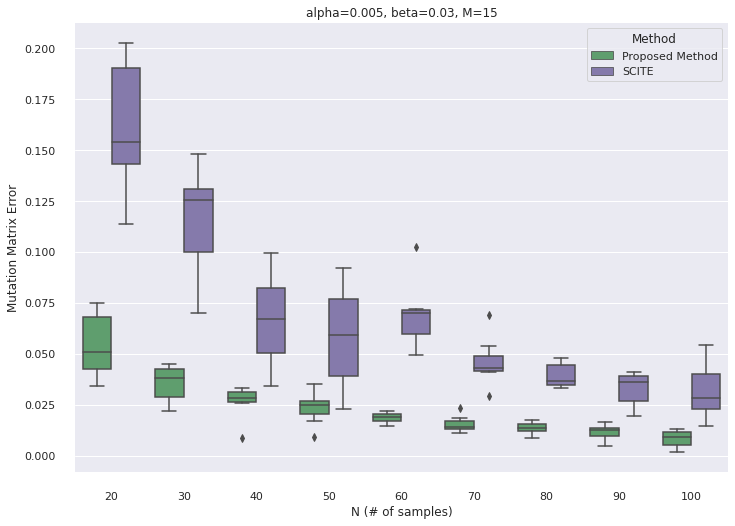
\includegraphics[width=0.7\textwidth]{img/chaps/er/comp_pm_scite}
	\caption{‌مقایسه روش پیشنهادی با روش پایه \lr{scite} با پارامترهای $\alpha=0.005, \beta=0.03, M=15$}
	\label{fig:sy_n_err_mean}
\end{figure}
همان‌طور که مشاهده می‌شود، با افزایش تعداد نمونه‌ها ضمن حفظ تعداد جهش‌ها، بازسازی به صورت ‌دقیق‌تری برای هر دو روش همراه است که روش پیشنهادی مشاهده می‌شود با تعداد تکرارهای برابر برای تعداد نمونه‌های یکسان از روش \lr{scite} پاسخ‌های دقیق‌تری ارائه می‌دهد.\\
همچنین تغییر پارامترها و اجرای مجدد خروجی تصویر \ref{fig:ch_er:comp_change_N} را به همراه دارد که در این تصویر، نمودار سمت چپ برابر میانگین خطای فاصله به ازای هر دو ژن در درخت بازسازی شده با درخت واقعی می‌باشد. همچنین در نمودار سمت راست نیز میانگین خطا نمایش داده شده است که این معیار خطا تابعی از خطای اصلی است که برای اینکه در تصاویر به همراه معیار فاصله در یک رنج قرار بگیرند به صورت  
$\left(\left( -\sum\ln(P)\right)/A\right)^{1.3}$ مورد استفاده قرار گرفته است.
\\ در این نمودار نیز کاهش دقت بنظر می‌رسد با سرعت بیشتری برای روش پایه همراه است.
\begin{figure}[!ht]
	\centering
	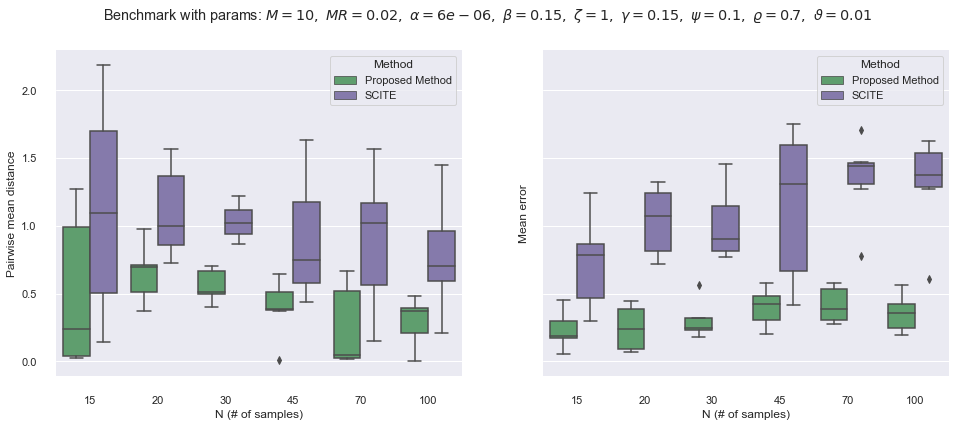
\includegraphics[width=\textwidth]{img/chaps/er/comp_change_N}
	\caption{‌مقایسه روش پیشنهادی با توجه به تغییر پارامتر $N$}
	\label{fig:ch_er:comp_change_N}
\end{figure}
\noindent
همچنین در نمودارهای تصویر \ref{fig:ch_er:comp_change_M} نتیجه اجرا برای حالتی است که تعداد جهش‌ها در حال افزایش است و نسبت $\frac{M}{N}=1.3$ در تمامی حالات برابر است. دیگر پارامترها بر روی تصویر ذکر شده قابل مشاهده است. در این نمودارها نیز با افزایش ابعاد ماتریس ورودی همچنان روش پیشنهادی نسبت به روش پایه از عملکرد مطلوب‌تری برخوردار است تا زمانی که تعداد جهش‌ها به $30$ می‌رسد که در این زمان خطای روش پایه‌ای بهتر از روش پیشنهادی بود که یکی از دلایل آن می‌تواند به اندازه کافی آموزش ندیدن شبکه باشد اما با این حال با توجه به این نکته که روش پیشنهادی فرض فقدان جهش را در خود دارد توانست همچنان میانگین فواصل بهتری را بین جفت جهش‌ها در درخت حاصل کند.
\begin{figure}[!ht]
	\centering
	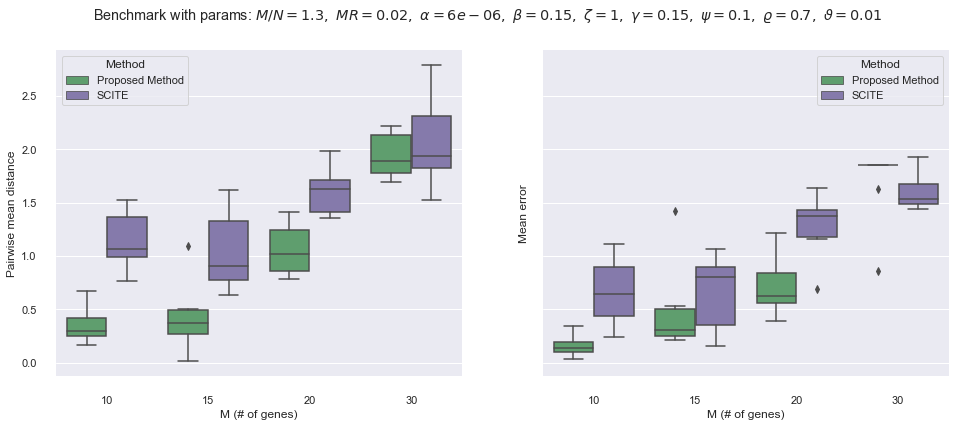
\includegraphics[width=\textwidth]{img/chaps/er/comp_change_M}
	\caption{‌مقایسه روش پیشنهادی با توجه به تغییر پارامتر $M$}
	\label{fig:ch_er:comp_change_M}
\end{figure}
\noindent
پس از مشاهده نتایج با توجه به تغییرات تعداد جهش‌ها و نمونه‌ها (ابعاد ماتریس) حال به بررسی تغییرات دیگر پارامترها خواهیم پرداخت. در ادامه نمودار شکل \label{fig:ch_er:comp_change_alpha} تغییرات خطا و میانگین فواصل بین ژن‌ها را با توجه به تغییر پارامتر $\alpha$ نمایش می‌دهد.

\begin{figure}[!ht]
	\centering
	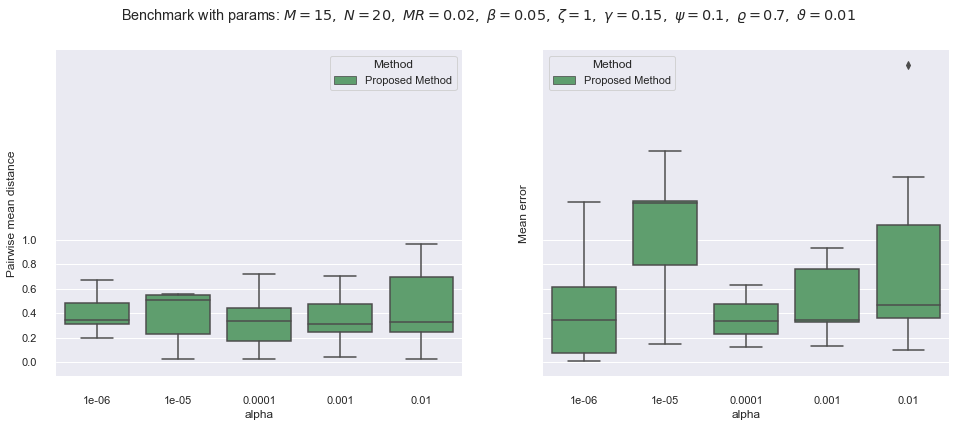
\includegraphics[width=\textwidth]{img/chaps/er/comp_change_alpha}
	\caption{‌مقایسه روش پیشنهادی با توجه به تغییر پارامتر $\alpha$}
	\label{fig:ch_er:comp_change_alpha}
\end{figure}
\noindent
در این شکل با توجه به این‌که مقدار $\alpha$ عدد کوچکی است، تغییرات ایجاد شده توسط آن در ماتریس ورودی برای الگوریتم پیشنهادی نیز به طبع کم تاثیر خواهد بود اما در نهایت با کمی دقت قابل استنتاج است که این افزایش با شیب کمی به افزایش خطا و کاهش دقت منجر خواهد شد.\\
به همین ترتیب نتایج برای تغییرات پارمتر $\beta$ نیز در شکل \ref{fig:ch_er:comp_change_beta} قابل مشاهده می‌باشد.

\begin{figure}[!ht]
	\centering
	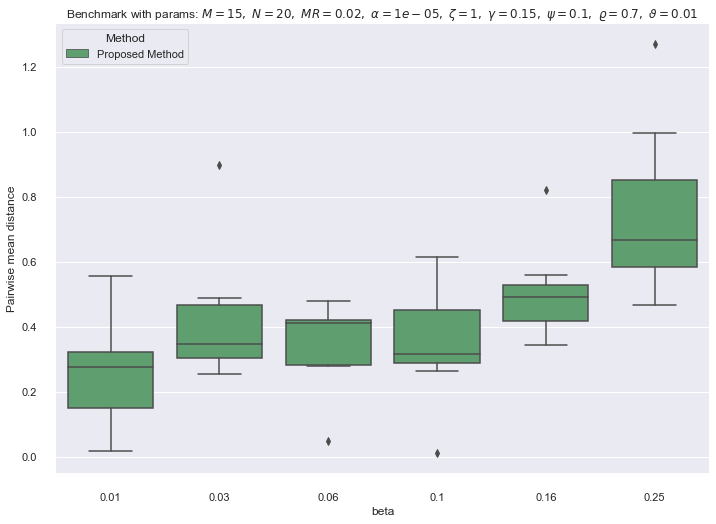
\includegraphics[width=0.75\textwidth]{img/chaps/er/comp_change_beta}
	\caption{‌مقایسه روش پیشنهادی با توجه به تغییر پارامتر $\beta$}
	\label{fig:ch_er:comp_change_beta}
\end{figure}
\noindent
اما به جز پارامترها که در روابط مد‌ل‌سازی شده‌اند یکی از مشکلات اصلی وجود داده‌های از دست رفته بود که دو رویکرد برای مدیریت آن‌ها مطرح کردیم. در تصاویر \ref{fig:ch_er:comp_change_MR_pwd} و \ref{fig:ch_er:comp_change_MR_me} نتایج حال از این دو رویکرد نشان داده شده است.

\begin{figure}[!ht]
	\centering
	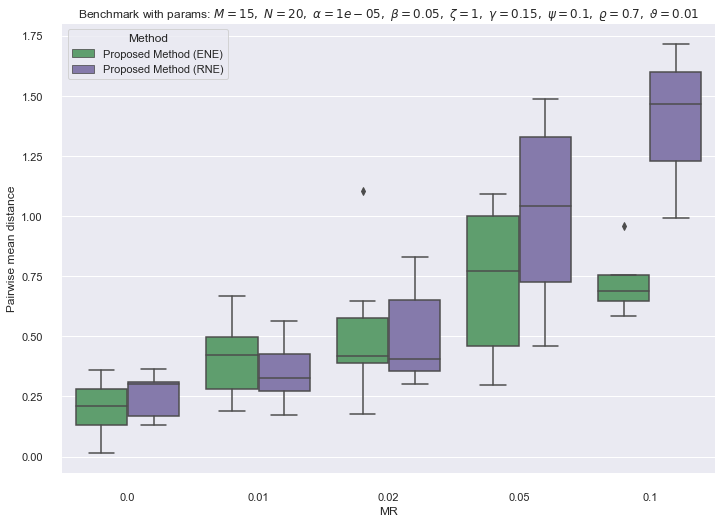
\includegraphics[width=0.75\textwidth]{img/chaps/er/comp_change_MR_pwd}
	\caption{‌مقایسه روش پیشنهادی با توجه به تغییر پارامتر $MR$ در دقت میانگین فواصل بین جهش‌ها در درخت فیلوژنی}
	\label{fig:ch_er:comp_change_MR_pwd}
\end{figure}
\begin{figure}[!ht]
	\centering
	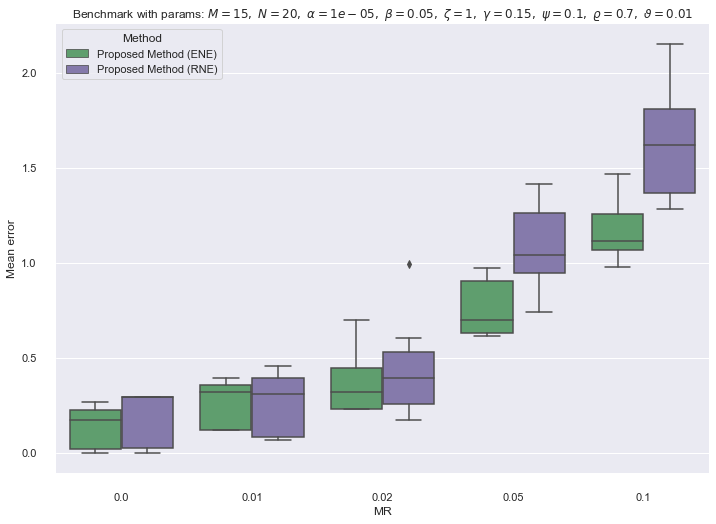
\includegraphics[width=0.75\textwidth]{img/chaps/er/comp_change_MR_me}
	\caption{‌مقایسه روش پیشنهادی با توجه به تغییر پارامتر $MR$ در مقدار میانگین خطا}
	\label{fig:ch_er:comp_change_MR_me}
\end{figure}
\noindent
همان‌گونه که در این دو تصویر ذکر شده هنگامی که نرخ داده‌های از دست رفته کم است هر دو حالت تقریبا عملکردی مشابه دارند. زیرا که پایین بودن این نرخ به منزله کمتر بودن تعداد داده‌های نامعلوم است که در این تعدادهای کم تفاوت مشخص نیست و خطاهای بوجود آمده نیز در قالب همان پارامترهای $\alpha$ و $\beta$ خود را نشان می‌دهد و مقادیر آن‌ها را نیز برای داده‌ها خراب نمی‌کند. اما رفته رفته هرچه این نرخ افزایش پیدا می‌کند، این اختلاف بیشتر شده و تاثیر خود را در رویکردهای مختلف بازسازی نمایش می‌دهد.

\subsection{نتایج بر روی داده‌های حقیقی}
در نهایت در این بخش روش پیشنهادی خود را بر روی دادگان حقیقی \cite{davis2016computing} اجرا کردیم که نتیجه بدست آمده از آن در شکل \ref{fig:ch_er:pm_tree} قابل مشاهده است.

\begin{figure}[!ht]
	\centering
	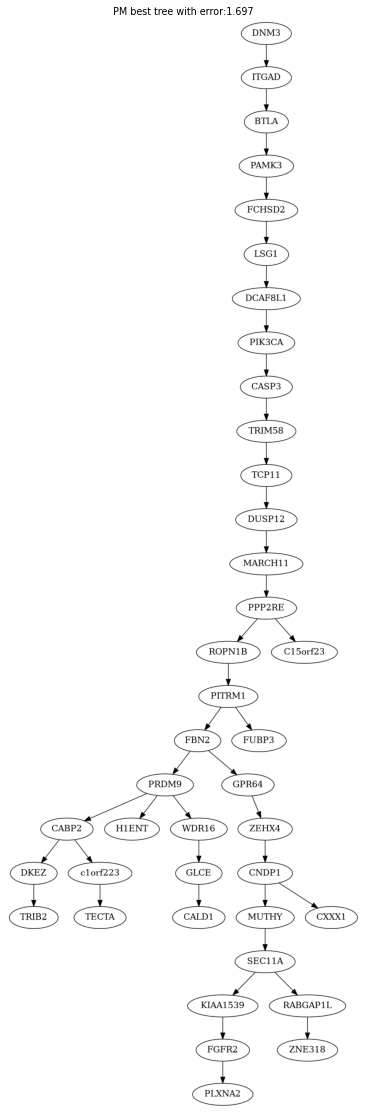
\includegraphics[width=0.4\textwidth]{img/chaps/er/pm2}
	\caption{درخت بدست داده‌های حقیقی مورد استفاده مقاله \cite{davis2016computing} توسط روش پیشنهادی}
	\label{fig:ch_er:pm_tree}
\end{figure}
\noindent
پارامترهای مورد استفاده برای این دادگان برابر با $\alpha=0.015$ و $\beta=0.13$ بودند. همچنین نتیجه بدست آمده بهترین نتیجه ممکن برای اجرای 100 بار الگوریتم به ازای ترکیب دو جهش مختلف جهت در مجموعه جهش‌های قابل حذف می‌باشد. ساختار درخت ارائه شده توسط خود مقاله نیز در شکل \ref{fig:ch_er:navin_tree} قابل مشاهده است.

\begin{figure}[!ht]
	\centering
	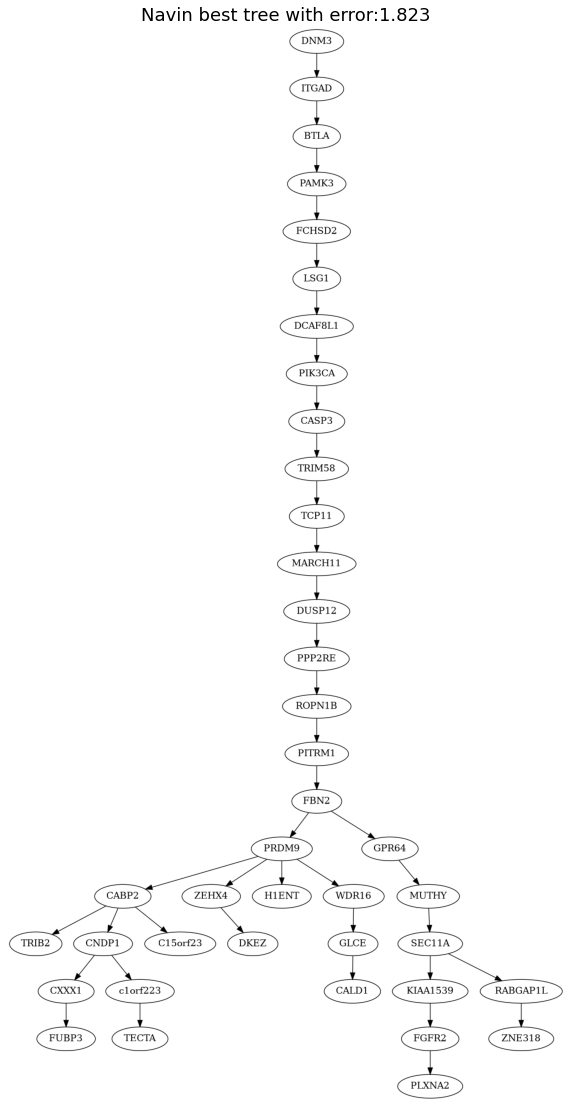
\includegraphics[width=0.6\textwidth]{img/chaps/er/navin}
	\caption{درخت بدست آمده در مقاله \lr{SCITE}}
	\label{fig:ch_er:navin_tree}
\end{figure}
\noindent
همان‌طور که مشخص است مقدار خطای بدست آمده برای خروجی الگوریتم پیشنهادی بهتر (کمتر) از خطای درخت \lr{SCITE} می‌باشد.
